%% USPSC-modelo-ICMCe.tex
% ---------------------------------------------------------------
% USPSC: Modelo de Trabalho Acadêmico (tese de doutorado, dissertacao de
% mestrado e trabalhos monograficos em geral) em conformidade com 
% ABNT NBR 14724:2011: Informação e documentação - Trabalhos acadêmicos -
% Apresentação
%----------------------------------------------------------------
%% Esta é uma customização do abntex2-modelo-trabalho-academico.tex de v-1.9.5 laurocesar 
%% para as Unidades do Campus USP de São Carlos:
%% EESC - Escola de Engenharia de São Carlos
%% IAU - Instituto de Arquitetura e Urbanismo
%% ICMC - Instituto de Ciências Matemáticas e de Computação
%% IFSC - Instituto de Física de São Carlos
%% IQSC - Instituto de Química de São Carlos
%%
%% Este trabalho utiliza a classe USPSC (USPSC.cls e USPSC1.cls) que é mantida 
%% pela seguinte equipe:
%% 
%% Coordenação e Programação:
%%   - Marilza Aparecida Rodrigues Tognetti - marilza@sc.usp.br (PUSP-SC)
%%   - Ana Paula Aparecida Calabrez - aninha@sc.usp.br (PUSP-SC)
%% Normalização:
%%   - Brianda de Oliveira Ordonho Sigolo - brianda@usp.br (IAU)
%%   - Eduardo Graziosi Silva - edu.gs@sc.usp.br (EESC)
%%   - Eliana de Cássia Aquareli Cordeiro - eliana@iqsc.usp.br (IQSC)
%%   - Flávia Helena Cassin - cassinp@sc.usp.br (EESC)
%%   - Maria Cristina Cavarette Dziabas - mcdziaba@ifsc.usp.br (IFSC)
%%   - Regina Célia Vidal Medeiros - rcvmat@icmc.usp.br (ICMC)
%%
%% Os modelos desenvolvidos utilizam diversos arquivos relacionado em 
%% 2.1 Pacote USPSC: Classe USPSC e modelos de trabalhos acadêmicos	do Tutorial do Pacote 
%%  USPSC para modelos de trabalhos de acadêmicos em LaTeX - versão 3.2

%----------------------------------------------------------------
%% Sobre a classe abntex2.cls:
%% abntex2.cls, v-1.9.5 laurocesar
%% Copyright 2012-2015 by abnTeX2 group at https://www.abntex.net.br/ 
%%
%----------------------------------------------------------------

\documentclass[
% -- opções da classe memoir --
12pt,		% tamanho da fonte
openany,	% capítulos podem começar em qualquer página para reduzir páginas em branco
%twoside,  % para impressão em anverso (frente) e verso. Oposto a oneside - Nota: utilizar \imprimirfolhaderosto*
%oneside, % para impressão em páginas separadas (somente anverso) -  Nota: utilizar \imprimirfolhaderosto
oneside,
% inclua uma % antes do comando twoside e exclua a % antes do oneside 
a4paper,			% tamanho do papel. 
% -- opções da classe abntex2 --
chapter=TITLE,		% títulos de capítulos convertidos em letras maiúsculas
% -- opções do pacote babel --
english,			% o último idioma é o principal do documento
french,				% idioma adicional para hifenização
spanish,			% idioma adicional para hifenização
brazil				% idioma adicional para hifenização 
% {classe/USPSC} configura o cabeçalho contendo apenas o número da página
]{classe/USPSC}
%]{classe/USPSC1}
% Inclua % antes de ]{classe/USPSC} e retire a % antes de %]{classe/USPSC1} para utilizar o
% cabeçalho diferenciado para as páginas pares e ímpares:
%- páginas ímpares: com seções ou subseções e o número da página
%- páginas pares: com o número da página e o título do capítulo 
% ---
% ---
% Pacotes básicos - Fundamentais 
% ---
\usepackage[T1]{fontenc}		% Seleção de códigos de fonte.
\usepackage[utf8]{inputenc}		% Codificação do documento (conversão automática dos acentos)
%\usepackage{lmodern}			% Usa a fonte Latin Modern
% Para utilizar a fonte Times New Roman, inclua uma % no início do comando acima  "\usepackage{lmodern}"
% Abaixo, tire a % antes do comando  \usepackage{times}
\usepackage{times}		    	% Usa a fonte Times New Roman (ABNT NBR 14724)
% Para usar a fonte , lembre-se de tirar a % do comando %\renewcommand{\ABNTEXchapterfont}{\rmfamily}, localizado mais abaixo, logo após "Outras opções para nota de rodapé no Sistema Numérico"
\usepackage{lastpage}			% Usado pela Ficha catalográfica
\usepackage{indentfirst}		% Indenta o primeiro parágrafo de cada seção.
\usepackage{color}				% Controle das cores
\usepackage{graphicx}			% Inclusão de gráficos
\usepackage{float} 				% Fixa tabelas e figuras no local exato
\usepackage{amsmath}			% Ambientes matemáticos (equation*, cases, etc.)
\usepackage{chemfig}            % Para escrever reações químicas
\usepackage{tikz}				% Para escrever reações químicas e outros
\usetikzlibrary{positioning,arrows.meta,shapes.geometric,fit,backgrounds}
\usepackage{microtype} 			% para melhorias de justificação
\usepackage{pdfpages}
\usepackage{makeidx}            % para gerar índice remissivo
\usepackage{hyphenat}          % Pacote para retirar a hifenizacao DO TEXTO
\usepackage[absolute]{textpos} % Pacote permite o posicionamento do texto
\usepackage{eso-pic}           % Pacote para incluir imagem de fundo
\usepackage{makebox}           % Pacote para criar caixa de texto
% ---

% ---
% Configurações globais de formatação
% ---
% Tamanho global de fonte monoespaçada (regra "CSS-like").
% Computer Modern Typewriter a 12pt fica largo demais e força quebras feias.
% Mudar \monospacesize aqui afeta TODO uso de fonte monoespaçada no PDF:
% \texttt, \path, \url, \verb, \ttfamily, ambientes verbatim, lstlisting etc.
% Valores típicos: \small (≈10.95pt), \footnotesize (≈10pt), \scriptsize (≈8pt).
\newcommand{\monospacesize}{\footnotesize}

% Hook global: toda chamada a \ttfamily passa também a aplicar \monospacesize.
% Como todas as variantes monoespaçadas (texttt, path, url, verb, verbatim,
% lstlisting, ...) terminam invocando \ttfamily, esta única regra cobre o PDF
% inteiro.
\let\origttfamily\ttfamily
\renewcommand{\ttfamily}{\origttfamily\monospacesize}

% url.sty / hyperref usam \UrlFont para \url e \path: rotear via \monospacesize.
\renewcommand{\UrlFont}{\monospacesize\origttfamily}
\makeatletter
\g@addto@macro{\UrlBreaks}{\do\/\do\-\do\_\do\.\do\:}
\makeatother

% ---
% Pacotes de citações
% Citações padrão ABNT
% ---
% Sistemas de chamada: autor-data ou numérico.
% Sistema autor-data
\usepackage[alf, abnt-emphasize=bf, abnt-thesis-year=both, abnt-repeated-author-omit=no, abnt-last-names=abnt, abnt-etal-cite=3, abnt-etal-list=3, abnt-etal-text=it, abnt-and-type=e, abnt-doi=doi, abnt-url-package=none, abnt-verbatim-entry=no]{abntex2cite}
%\bibliographystyle{classe/abntex2-alf-USPSC}
% Se o idioma for o inglês, inclua % no comando acima e exclua o % do comando abaixo
\bibliographystyle{classe/abntex2-alfeng-USPSC}

% Para o IQSC, que indica todos os autores nas referências, incluir % no início dos comandos acima e retirar a % dos comandos abaixo
%\usepackage[alf, abnt-emphasize=bf, abnt-thesis-year=both, abnt-repeated-author-omit=no, abnt-last-names=abnt, abnt-etal-cite=3, abnt-etal-list=0, abnt-etal-text=it, abnt-and-type=e, abnt-doi=doi, abnt-url-package=none, abnt-verbatim-entry=no]{abntex2cite}
%\bibliographystyle{classe/abntex2-alf-USPSC}
% Se o idioma for o inglês, exclua % no comando acima ou do comando abaixo
%\bibliographystyle{classe/abntex2-alfeng-USPSC}

% Sistema Numérico
% Para citações numéricas, sistema adotado pelo IFSC, incluir % no início dos comandos acima e retirar a % dos comandos abaixo
%\usepackage{cite}              % agrupa citações numéricas consecutivas
%\usepackage[num, abnt-emphasize=bf, abnt-thesis-year=both, abnt-repeated-author-omit=no, abnt-last-names=abnt, abnt-etal-cite=3, abnt-etal-list=3, abnt-etal-text=it, abnt-and-type=e, abnt-doi=doi, abnt-url-package=none, abnt-verbatim-entry=no]{abntex2cite}
%\bibliographystyle{classe/abntex2-num-USPSC}
% Se o idioma for o inglês, exclua % no comando acima ou do comando abaixo
%\bibliographystyle{classe/abntex2-numeng-USPSC}

% Complementarmente, verifique as instruções abaixo sobre os Pacotes de Nota de rodapé
% ---
% Pacotes de Nota de rodapé
% Configurações de nota de rodapé

% O presente modelo adota o formato numérico para as notas de rodapés quando utiliza o sistema de chamada autor-data para citações e referências. Para utilizar o sistema de chamada numérico para citações e referências, habilitar um dos comandos abaixo.
% Há diversa opções para nota de rodapé no Sistema Numérico.  Para o IFSC, habilitade o comando abaixo.

%\renewcommand{\thefootnote}{\fnsymbol{footnote}}  %Comando para inserção de símbolos em nota de rodapé

% Outras opções para nota de rodapé no Sistema Numérico:
%\renewcommand{\thefootnote}{\alph{footnote}}      %Comando para inserção de letras minúscula em nota de rodapé
%\renewcommand{\thefootnote}{\Alph{footnote}}      %Comando para inserção de letras maiúscula em nota de rodapé
%\renewcommand{\thefootnote}{\roman{footnote}}     %Comando para inserção de números romanos minúsculos  em nota de rodapé
%\renewcommand{\thefootnote}{\Roman{footnote}}     %Comando para inserção de números romanos minúsculos  em nota de rodapé

\renewcommand{\footnotesize}{\small} %Comando para diminuir a fonte das notas de rodapé
%Para utilizar a fonte Times New Roman, inclua retire % do início do comando abaixo
\renewcommand{\ABNTEXchapterfont}{\rmfamily}

% ---
% Pacote para agrupar a citação numérica consecutiva
% Quando for adotado o Sistema Numérico, a exemplo do IFSC, habilite 
% o pacote cite abaixo retirando a porcentagem antes do comando abaixo
%\usepackage[superscript]{cite}	

% ---
% Pacotes adicionais, usados apenas no âmbito do Modelo Canônico do abnteX2
% ---
\usepackage{lipsum}				% para geração de dummy text
% ---

% pacotes de tabelas
\usepackage{multicol}	% Suporte a mesclagens em colunas
\usepackage{multirow}	% Suporte a mesclagens em linhas
\usepackage{longtable}	% Tabelas com várias páginas
\usepackage{threeparttablex}    % notas no longtable
\usepackage{array}

% ----
% Compatibilização com a ABNT NBR 6023:2018 e 10520:2023
% Para tirar <> da URL e tornar as expressões latinas em itálico
\usepackage{classe/ABNT6023-10520}
% As demais compatibilizações estão nos arquivos abntex2-alf-USPSC.bst,abntex2-alfeng-USPSC.bst, abntex2-num-USPSC.bst e abntex2-numeng-USPSC.bst, dependendo do idioma do textos e se o sistemas de chamada for autor-data ou numérico, conforme explicitado acima.
% ----

% ---
% DADOS INICIAIS - Define sigla com título, área de concentração e opção do Programa 
% Consulte a tabela referente aos Programas, áreas e opções de sua unidade contante do
% arquivo USPSC-Siglas estabelecidas para os Programas de Pós-Graduação nos APÊNDICES B-J
\siglaunidade{ICMC}
\programa{MBAIAe} % MBA in Artificial Intelligence and Big Data (English)
% Os demais dados deverão ser fornecidos no arquivo USPSC-pre-textual-UUUU ou USPSC-TCC-pre-textual-UUUU, onde UUUU é a sigla da Unidade. 
% Exemplo:USPSC-pre-textual-IFSC.tex
% ---
% Configurações de aparência do PDF final
% alterando o aspecto da cor azul
\definecolor{blue}{RGB}{41,5,195}

% informações do PDF
\makeatletter
\hypersetup{
	%pagebackref=true,
	pdftitle={\@title}, 
	pdfauthor={\@author},
	pdfsubject={\imprimirpreambulo},
	pdfcreator={LaTeX with abnTeX2},
	pdfkeywords={abnt}{latex}{abntex}{USPSC}{trabalho acadêmico}, 
	colorlinks=true,       		% false: boxed links; true: colored links
	linkcolor=black,          	% color of internal links
	citecolor=black,        		% color of links to bibliography
	filecolor=black,      		% color of file links
	urlcolor=black,
	%Para habilitar as cores dos links, retire a % antes dos comandos abaixo e inclua a % antes das 4 linhas de comando acima 
	%linkcolor=blue,            	% color of internal links
	%citecolor=blue,        		% color of links to bibliography
	%filecolor=magenta,      		% color of file links
	%urlcolor=blue,
	bookmarksdepth=4	
}
\makeatother
% --- 
% --- 
% Espaçamentos entre linhas e parágrafos 
% --- 

% O tamanho do parágrafo é dado por (ABNT NBR 14724: 1.25 cm):
\setlength{\parindent}{1.25cm}

% Controle do espaçamento entre um parágrafo e outro
% (ABNT NBR 14724: corpo do texto sem espaço extra entre parágrafos):
\setlength{\parskip}{0pt}

% ---
% compila o sumário e índice
\makeindex
% ---

% ----
% Início do documento
% ----
\begin{document}
	
	% Seleciona o idioma do documento (conforme pacotes do babel)
	%\selectlanguage{brazil}
	% Se o idioma do texto for inglês, inclua uma % antes do 
	%      comando \selectlanguage{brazil} e 
	%      retire a % antes do comando abaixo
	\selectlanguage{english}
	
	% Retira espaço extra obsoleto entre as frases.
	\frenchspacing 
	
	% --- Formatação dos Títulos
	\renewcommand{\ABNTEXchapterfontsize}{\fontsize{12}{12}\bfseries}
	\renewcommand{\ABNTEXsectionfontsize}{\fontsize{12}{12}\bfseries}
	\renewcommand{\ABNTEXsubsectionfontsize}{\fontsize{12}{12}\normalfont}
	\renewcommand{\ABNTEXsubsubsectionfontsize}{\fontsize{12}{12}\normalfont}
	\renewcommand{\ABNTEXsubsubsubsectionfontsize}{\fontsize{12}{12}\normalfont}

% =========================================================================
% PRE-TEXTUAL ELEMENTS
% =========================================================================

% Cover (ICMC)
%% pre/cover.tex
\AddToShipoutPicture{\BackgroundPic}
%-------------
\begin{minipage}[c]{144mm}
   \centering
   \begin{textblock*}{144mm}(61mm,65mm)
   \vspace*{1,2cm}
   \linespread{0.5}
   \ABNTEXchapterfont\bfseries\Large
   \textcolor{capa-azul}{\nohyphens{\imprimirtitulo}}
   \end{textblock*}
\end{minipage}
\vfill
\vspace*{5cm}
\begin{minipage}[t][65mm][t]{125mm}
   \begin{textblock*}{130mm}(81mm,123mm)
      \ABNTEXchapterfont\bfseries\Large
      \textcolor{capa-azul}{\nohyphens{\imprimirautor}} 
      \vfill
      \vspace{9pt}
      \ABNTEXsubsectionfontsize\small
      \renewcommand{\ABNTEXsubsectionfontsize}{\fontsize{10}{6}\normalfont}
      \ABNTEXsubsectionfontsize 
      \textcolor{capa-azul}{\nohyphens{\imprimirnotacapaicmc}}
      \renewcommand{\ABNTEXsubsectionfontsize}{\fontsize{12}{12}\normalfont}
   \end{textblock*}	
\end{minipage} 
% ---

\AddToShipoutPicture{\BackgroundBranco}

\includepdf{pre/blank-page.pdf}

% Title page (twoside variant)
\imprimirfolharostocar*

% Cataloging sheet (provided by the library as a PDF after submission).
% Re-enable the \includepdf line once catalog-card.pdf is available.
% \includepdf{pre/catalog-card.pdf}
%% pre/catalog-card.tex
%% Cataloging-card page (ficha catalogr\'afica) aligned with the layout of
%% Bruna Magrini da Cruz's 2025 ICMC-USP MBA TCC. Layout: PT header (sans,
%% centered, 3 lines), box centered below in typewriter font, ICMC
%% librarian credit at the bottom-left in sans-serif. The "I AUTHORIZE"
%% statement is intentionally omitted from this page (it does not appear
%% on Bruna's ficha catalogr\'afica; if the institution later requires it
%% on this page, restore the \imprimirnotaautorizacao line at the top).
\begin{fichacatalografica}

\begin{center}
  {\sffamily\small\imprimirnotabib}
\end{center}

\vspace*{0.6cm}

\begin{center}
  \begin{tabular}{|p{0.9cm} p{8.7cm}|}
    \hline
    \multicolumn{2}{|l|}{\scriptsize\ttfamily~} \\
                            & \scriptsize\ttfamily\imprimirautorficha \\
    \scriptsize\ttfamily\imprimircutter &
        \scriptsize\ttfamily\hspace{0.4cm}\imprimirtitulo~/~\imprimirautor~;~\imprimirorientadorcorpoficha. --~\imprimirlocal, \imprimirdata. \\
                            & \scriptsize\ttfamily\hspace{0.4cm}\pageref{LastPage}~p. \\
    \multicolumn{2}{|l|}{\scriptsize\ttfamily~} \\
                            & \scriptsize\ttfamily\hspace{0.4cm}Trabalho de conclus\~ao de curso (MBA em Intelig\^encia Artificial e Big Data)~--~Instituto de Ci\^encias Matem\'aticas e de Computa\c{c}\~ao, Universidade de S\~ao Paulo, \imprimirdata. \\
    \multicolumn{2}{|l|}{\scriptsize\ttfamily~} \\
                            & \scriptsize\ttfamily\hspace{0.4cm}1.~Algorithmic trading.~2.~Foreign exchange (forex).~3.~Natural language processing.~4.~Sentiment analysis.~5.~Geopolitical events.~6.~Financial machine learning.~I.~\imprimirorientadorficha.~II.~T\'itulo. \\
    \multicolumn{2}{|l|}{\scriptsize\ttfamily~} \\
    \hline
  \end{tabular}
\end{center}

% Librarian credit (e.g.\ "Bibliotec\'arios respons\'aveis ...") is
% intentionally omitted at this stage. The ICMC Library generates the
% official ficha catalogr\'afica with the librarian credit after the
% manuscript is deposited; at that point replace this entire file with
% \includepdf{pre/catalog-card.pdf} from the main.tex pre-textual block.

\end{fichacatalografica}



% Additional title page in Portuguese (ABNT NBR 14724 / USP MBA convention).
% Title stays in English; preamble, concentration area, advisor label, and the
% "Versão original" note appear in pt-BR. Same layout as Bruna Magrini's
% well-evaluated 2025 ICMC-USP TCC.
\imprimirfolhaderostoadic*

% Errata
%%% pre/errata.tex
\begin{errata}
    %\OnehalfSpacing
    The errata is an optional element consisting of a list of errors in the work, preceded by the pages and lines where they occur and followed by the corresponding corrections. It must be inserted right after the title page and contain the reference of the work to ease identification, as per ABNT NBR 14724.

    Errata template:

    \begin{flushleft}
        \setlength{\absparsep}{0pt}
        \SingleSpacing
        \imprimirautorabr~ ~\textbf{\imprimirtituloresumo}.	\imprimirdata. \pageref{LastPage} p.
        \imprimirtipotrabalho~-~\imprimirinstituicao, \imprimirlocal, \imprimirdata.
    \end{flushleft}
    \vspace{\onelineskip}
    \OnehalfSpacing
    \center
    \textbf{ERRATA}
    \vspace{\onelineskip}
    \OnehalfSpacing
    \begin{table}[htb]
        \center
        \footnotesize
        \begin{tabular}{p{2cm} p{2cm} p{4cm} p{4cm} }
            \hline
            \textbf{Page} & \textbf{Line}  & \textbf{Where it reads}  & \textbf{Read}  \\
            \hline
            1 & 10 & auto-conclavo & autoconclavo\\
            \hline
        \end{tabular}
    \end{table}
\end{errata}



% Approval sheet (signed PDF generated after the defense).
% Re-enable the \includepdf line once approval-sheet.pdf is available.
% \includepdf{pre/approval-sheet.pdf}
%% pre/approval-sheet.tex
%% Alternative to the scanned approval sheet PDF.
\begin{folhadeaprovacao}
  \begin{center}
       {\ABNTEXchapterfont\bfseries\large\imprimirautor}
     \vspace*{2cm}

    \begin{center}
      \ABNTEXchapterfont\bfseries\Large\imprimirtitulo
    \end{center}
        \vspace*{2cm}
        \hspace{.45\textwidth}
    \begin{minipage}{.5\textwidth}
        \imprimirpreambulo
    \end{minipage}
        \vspace*{2cm}
    \end{center}

  \begin{center}
      {\ABNTEXchapterfont\bfseries\large\ {Defense date: \rule{4cm}{0.4pt}} \\}
        \vspace*{\fill}
      {\ABNTEXchapterfont\bfseries\large\ {Examination committee:} \\}

        \assinatura{\textbf{\imprimirorientador} \\}
        \renewcommand{\orientadorname}{Carolina Toledo Ferraz}

        \imprimirorientadorRotulo
        \par
        %\assinatura{\textbf{Professor} \\ Member 1}
        %\assinatura{\textbf{Professor} \\ Member 2}
        %\assinatura{\textbf{Professor} \\ Member 3}
        %\assinatura{\textbf{Professor} \\ Member 4}
        \vspace*{\fill}
       {\ABNTEXchapterfont\bfseries\large\imprimirlocal}
    \par
    {\ABNTEXchapterfont\bfseries\large\imprimirdata}
\end{center}
\end{folhadeaprovacao}



\includepdf{pre/blank-page.pdf}

% Dedication
%% pre/dedication.tex
\begin{dedicatoria}
	\vspace*{\fill}
	\centering
	\noindent
	{\itshape%
		I dedicate this work to my family, for their unwavering support, encouragement, and belief in me throughout this journey.\par

		To my friends, who stood by me with patience, motivation, and understanding during both the difficult and rewarding moments.\par

		To everyone who contributed, in any way, to the completion of this work, my heartfelt thanks.\par
	}
	\vspace*{\fill}
\end{dedicatoria}


% Acknowledgments
%%% pre/acknowledgments.tex
\begin{agradecimentos}
    First acknowledgment sentence ....

    Second sentence ....

    Other sentences ....

    Final sentence ....

\end{agradecimentos}



% Epigraph
%% pre/epigraph.tex
\begin{epigrafe}
    \vspace*{\fill}
    \begin{flushright}
        \textit{``If I have seen further it is by standing on the shoulders of giants.''\\
       Isaac Newton}
    \end{flushright}
\end{epigrafe}



% Abstract (English).
%% pre/abstract.tex
\begin{resumo}[Abstract]
 \begin{otherlanguage*}{english}
    \begin{flushleft}
        \setlength{\absparsep}{0pt}
        \SingleSpacing  		\imprimirautorabr~~\textbf{\imprimirtitleabstract}.	\imprimirdata.  \pageref{LastPage} p.
        \imprimirtipotrabalhoabs~-~\imprimirinstituicao, \imprimirlocal, 	\imprimirdata.
    \end{flushleft}
    \OnehalfSpacing
   This work investigates whether news-derived event features can improve the risk-adjusted performance of a Forex trading strategy beyond a price-only baseline. Although the title refers to AI-driven sentiment, the executed study tests GDELT coded-event intensity; article-level sentiment scoring was not executed. The question matters because the Forex market is strongly driven by news flow and macroeconomic information, yet the literature on text-based prediction of financial returns has concentrated on equities, leaving the asset class comparatively underexplored. The executed approach builds, on EUR/USD at minute resolution, a hybrid trading pipeline that combines technical signals with GDELT event-intensity features, fused into a single trade decision under strict point-in-time discipline and a conservative publication-to-use delay. Evaluation contrasts the hybrid against the price-only baseline under the same execution model, complemented by ablations, drift controls, multiple-comparisons checks and paired statistical tests. The hybrid strategy did not outperform the baseline in the tested configuration. The main contributions are a reproducible negative result showing that apparent profitability does not necessarily imply predictive ability, and a reusable methodology that subsequent work can extend with richer text sources, additional instruments and broader validation protocols.

   \vspace{\onelineskip}

   \noindent
   \textbf{Keywords}: algorithmic trading. forex. event features. GDELT. backtesting. reproducibility. financial machine learning.
 \end{otherlanguage*}
\end{resumo}


% ABNT NBR 14724 requires a Portuguese-language abstract (Resumo) on
% ICMC-USP MBA submissions, even when the body of the document is in English.
% pre/resumo.tex ships a pt-BR translation of the Abstract.
\renewcommand{\titleabstract}{Can AI-Driven Sentiment Improve Forex Trading?}
%% pre/resumo.tex
%% Portuguese-language abstract (Resumo) required by ABNT NBR 14724 and by
%% the ICMC-USP MBA submission rules, even though the body of the document
%% is in English. Mirrors pre/abstract.tex in content and ordering.
\setlength{\absparsep}{18pt}
\begin{resumo}[Resumo]
 \begin{otherlanguage*}{brazil}
    \begin{flushleft}
        \setlength{\absparsep}{0pt}
        \SingleSpacing
        \imprimirautorabr~~\textbf{\imprimirtituloresumo}.	\imprimirdata. \pageref{LastPage} p.
        \imprimirtipotrabalho~-~\imprimirinstituicao, \imprimirlocal, \imprimirdata.
    \end{flushleft}
    \OnehalfSpacing
    Este trabalho investiga se atributos de sentimento e de eventos derivados de t\'ecnicas de Processamento de Linguagem Natural (PLN) s\~ao capazes de melhorar o desempenho ajustado a risco de uma estrat\'egia de negocia\c{c}\~ao algor\'itmica no mercado de c\^ambio (Forex) em rela\c{c}\~ao a uma estrat\'egia de refer\^encia baseada apenas em pre\c{c}os. A pergunta \'e relevante porque o mercado de c\^ambio \'e fortemente influenciado por fluxos de not\'icias e por informa\c{c}\~ao macroecon\^omica; ainda assim, a literatura sobre previs\~ao de retornos financeiros a partir de texto tem se concentrado em mercados acion\'arios, deixando essa classe de ativos comparativamente menos explorada. A abordagem proposta constr\'oi, sobre dois pares principais de c\^ambio em resolu\c{c}\~ao de um minuto, uma estrat\'egia h\'ibrida que combina sinais t\'ecnicos com atributos de sentimento e de eventos extra\'idos de texto financeiro e de um \'indice p\'ublico de risco geopol\'itico, integrados em uma \'unica decis\~ao de negocia\c{c}\~ao sob disciplina temporal estrita (\emph{point-in-time}) e com um atraso conservador entre a publica\c{c}\~ao e o uso da informa\c{c}\~ao; as fontes de dados, os escoradores e os componentes de decis\~ao s\~ao detalhados no cap\'itulo de metodologia. A avalia\c{c}\~ao contrasta a estrat\'egia h\'ibrida com a estrat\'egia de refer\^encia baseada apenas em pre\c{c}os, em dados fora da amostra, sob custos de transa\c{c}\~ao realistas, complementada por um estudo de abla\c{c}\~ao que isola a contribui\c{c}\~ao marginal do canal textual e por um teste estat\'istico formal da diferen\c{c}a entre as distribui\c{c}\~oes de retornos. A contribui\c{c}\~ao \'e dupla: um teste emp\'irico e falsific\'avel da hip\'otese de que adicionar atributos textuais derivados de PLN melhora o desempenho ajustado a risco nos dois pares-alvo, e uma metodologia reutiliz\'avel que trabalhos subsequentes possam estender sem reimplementa\c{c}\~ao.

    \vspace{\onelineskip}

    \noindent
    \textbf{Palavras-chave}: negocia\c{c}\~ao algor\'itmica. mercado de c\^ambio (Forex). processamento de linguagem natural. an\'alise de sentimento financeiro. extra\c{c}\~ao de eventos. FinBERT. GDELT. risco geopol\'itico. \emph{backtesting}.
 \end{otherlanguage*}
\end{resumo}



% Lists - re-enable each block as the corresponding asset type starts to
% appear in the chapters. Figures: 2 TikZ diagrams in the body (ch.~3), so the
% list of figures is enabled. Tables: 4 in the body (one in ch.~2, three in
% ch.~3), so the list of tables is enabled.
\pdfbookmark[0]{\listfigurename}{lof}
\listoffigures*
\cleardoublepage

\pdfbookmark[0]{\listtablename}{lot}
\listoftables*
\cleardoublepage

% \pdfbookmark[0]{\listofquadroname}{loq}
% \listofquadro*
% \cleardoublepage

% pre/abbreviations.tex - List of abbreviations and acronyms used in this
% work. Grouped by domain (Forex / trading; NLP and AI; data and
% engineering; institutional) but rendered as a single alphabetical list,
% since that is what the abntex2 \siglas environment produces.
\begin{siglas}
    % --- Forex / trading / technical analysis ----------------------------
    \item[ADX] Average Directional Index (technical indicator)
    \item[ATR] Average True Range (volatility indicator)
    \item[BIS] Bank for International Settlements
    \item[BOJ] Bank of Japan
    \item[CAMEO] Conflict and Mediation Event Observations (event taxonomy)
    \item[ECB] European Central Bank
    \item[ECN] Electronic Communication Network
    \item[EUR] Euro (ISO 4217 currency code)
    \item[FOMC] Federal Open Market Committee
    \item[FX] Foreign Exchange
    \item[Forex] Foreign Exchange (market)
    \item[GBP] Pound Sterling (ISO 4217 currency code)
    \item[GPR] Geopolitical Risk (index of Caldara and Iacoviello)
    \item[HFT] High-Frequency Trading
    \item[JPY] Japanese Yen (ISO 4217 currency code)
    \item[MACD] Moving Average Convergence Divergence (technical indicator)
    \item[OHLC] Open, High, Low, Close (price-bar tuple)
    \item[OTC] Over-the-Counter (market)
    \item[P\&L] Profit and Loss
    \item[pip] Percentage in Point (smallest standard FX price increment)
    \item[RSI] Relative Strength Index (momentum oscillator)
    \item[USD] United States Dollar (ISO 4217 currency code)
    \item[ZN] CBOT Ten-Year U.S. Treasury Note futures (ticker)
    % --- AI / ML / NLP ---------------------------------------------------
    \item[AI] Artificial Intelligence
    \item[BERT] Bidirectional Encoder Representations from Transformers
    \item[BERTimbau] BERT pre-trained for Brazilian Portuguese
    \item[BPE] Byte-Pair Encoding (sub-word tokenization algorithm)
    \item[CBOW] Continuous Bag-of-Words (word2vec architecture)
    \item[FinBERT] Financial-domain fine-tuned BERT
    \item[FinGPT] Open-source financial Large Language Model
    \item[GloVe] Global Vectors for Word Representation
    \item[GPT] Generative Pre-trained Transformer
    \item[GPU] Graphics Processing Unit
    \item[LLM] Large Language Model
    \item[LSTM] Long Short-Term Memory (recurrent neural network cell)
    \item[ML] Machine Learning
    \item[MLM] Masked Language Modeling
    \item[NLP] Natural Language Processing
    \item[OOV] Out-Of-Vocabulary
    \item[OPRO] Optimization by PROmpting (LLM prompt-optimization method)
    \item[POS] Part-Of-Speech (tagging)
    \item[PLN] Processamento de Linguagem Natural (Portuguese for NLP)
    \item[RLHF] Reinforcement Learning from Human Feedback
    \item[RNN] Recurrent Neural Network
    \item[SHAP] SHapley Additive exPlanations (model-interpretation method)
    \item[SLM] Small Language Model
    \item[T5] Text-to-Text Transfer Transformer
    \item[TF] Term Frequency
    \item[TF--IDF] Term Frequency--Inverse Document Frequency
    % --- Data and engineering --------------------------------------------
    \item[API] Application Programming Interface
    \item[CC-News] Common Crawl News (corpus)
    \item[CSV] Comma-Separated Values (file format)
    \item[FNSPID] Financial News and Stock Price Integration Dataset
    \item[GDELT] Global Database of Events, Language and Tone
    \item[GKG] Global Knowledge Graph (GDELT 2.0 table)
    \item[GPL] GNU General Public License
    \item[HTTP] HyperText Transfer Protocol
    \item[LEAN] open-source algorithmic-trading engine maintained by QuantConnect
    \item[LGPL] GNU Lesser General Public License
    \item[MVP] Minimum Viable Product
    \item[OANDA] online Forex and CFD brokerage (proper name)
    \item[RAM] Random-Access Memory
    \item[REST] Representational State Transfer
    \item[SQL] Structured Query Language
    \item[YAML] YAML Ain't Markup Language (data-serialization format)
    % --- Institutional / academic ---------------------------------------
    \item[ABNT] Brazilian Association of Technical Standards
    \item[ICMC] Institute of Mathematics and Computer Sciences (USP)
    \item[MBA] Master of Business Administration
    \item[NBR] Norma Brasileira (Brazilian Standard)
    \item[USP] University of S\~ao Paulo
\end{siglas}


% pre/symbols.tex - List of mathematical symbols used in this work.
% Grouped by domain (price/market, model, evaluation, NLP/attention) but
% rendered as a single ordered list by the abntex2 \simbolos environment.
\begin{simbolos}
  % --- Market and price -------------------------------------------------
  \item[$P_{XY,t}$] Price of currency pair $XY$ at time $t$
  \item[$t$] Discrete time index (minute bar)
  \item[$H$] Forecast horizon (number of bars into the future)
  % --- Strategy state at time $t$ --------------------------------------
  \item[$\hat{p}_t$] Calibrated probability output of the meta-learner at time $t$
  \item[$\theta_{\text{high}}$] Upper decision threshold on $\hat{p}_t$
  \item[$\theta_{\text{low}}$] Lower decision threshold on $\hat{p}_t$
  \item[$r_t$] Trend-regime label at time $t$ (bull, bear, sideways)
  \item[$v_t$] Event-veto flag from the news-context filter at time $t$
  % --- Cross-validation ------------------------------------------------
  \item[$k$] Number of folds in combinatorial purged $k$-fold cross-validation
  % --- Transformer / attention -----------------------------------------
  \item[$X$] Input token sequence to a Transformer block
  \item[$Q$] Query matrix in scaled dot-product attention
  \item[$K$] Key matrix in scaled dot-product attention
  \item[$V$] Value matrix in scaled dot-product attention
  \item[$W^Q, W^K, W^V$] Learned projection matrices for $Q$, $K$, $V$
  \item[$d_k$] Dimensionality of the key vectors (attention scaling factor)
  \item[$h$] Number of parallel attention heads in multi-head attention
  \item[$n$] Length of a sub-word $n$-gram in BPE tokenization
\end{simbolos}



% Table of contents
\pdfbookmark[0]{\contentsname}{toc}
\tableofcontents*
\cleardoublepage

% =========================================================================
% TEXTUAL ELEMENTS
% =========================================================================
\textual

\chapter{Introduction} \label{cap:introduction}

The foreign exchange market (Forex or FX) trades roughly USD 7.5 trillion a day across spot, swap and derivative instruments \cite{bis2022triennial}. A market of that magnitude does not respond to price charts alone. Currency pairs react, often within seconds, to central-bank decisions, military escalation, sanctions, supply-chain shocks and political instability. Market participants able to ingest, interpret and act on such textual information faster than the average competitor retain a measurable advantage.

Trading strategies that rely exclusively on technical indicators applied to OHLC price bars \cite{murphy1999technical} have been documented to perform adequately under stable price regimes and to deteriorate when news flow, rather than price flow, drives the market. Modern Natural Language Processing (NLP) and the public release of finance-tuned language models \cite{araci2019finbert,yang2020finbert,wu2023bloomberggpt,liu2023fingpt} have substantially lowered the cost of revisiting that limitation empirically. Although the title refers to \emph{AI-driven sentiment}, the executed study tests GDELT coded-event intensity; it does not execute article-level sentiment scoring. The present work therefore investigates a hybrid trading pipeline that complements price-based signals with news-derived event features, evaluated under a strict backtesting protocol on historical data.

\section{Theme and Problem} \label{sec:theme-problem}

The theme is the integration of news-derived information into algorithmic decision-making for Forex. The driving research question is the following:

\begin{quote}
Can news-derived event features improve risk-adjusted Forex performance over a price-only baseline?
\end{quote}

\subsection*{Hypothesis} \label{sec:hypothesis}
The central premise of this study, that adding news-derived event features to a competitive price-only baseline improves risk-adjusted Forex performance, is a \textit{hypothesis}, not an established result. The evidence reviewed in Section~\ref{sec:justification} makes the premise plausible, but plausibility is not proof. The empirical apparatus developed in this work subjects that premise to a falsifiable test rather than presupposing it. The research question is therefore operationalized as a single hypothesis:
\begin{description}
  \item[\textbf{H1}] On the executed EUR/USD evaluation window, the hybrid
  strategy of Chapter~\ref{cap:methodology} produces a statistically meaningful
  improvement over the price-only baseline under the same data, execution model,
  costs and paired statistical test.
\end{description}
H1 is referenced under an explicit accept/reject criterion in
Section~\ref{sec:final-remarks} of the conclusion, derived from the evidence
reported in Chapter~\ref{cap:experimental-evaluation}. A rejection constitutes
a valid and reportable outcome: it would establish that, under this protocol
and on this pair, the event channel does not yield a statistically
meaningful improvement over the price-only baseline. Such a negative finding
is itself a contribution, and motivates stating the hypothesis in a form that
the evidence can refute.

The problem has three methodological parts. First, event data at currency-grade scale must be collected and time-aligned with FX prices \cite{leetaru2013gdelt}. Second, coded events must be transformed into numeric features that retain financially meaningful signal without leaking future information into past decisions \cite{loughran2011liability,tetlock2007giving}. Third, the combined feature space must drive entries, exits and position sizing in a way that remains auditable under regime change \cite{lopezdeprado2018advances}.

\section{Justification and Motivation} \label{sec:justification}

Three lines of reasoning motivate this investigation.

The empirical case is decades old, although most of the supporting evidence comes from equities rather than Forex. \citeonline{tetlock2007giving}, working on the US equity market, demonstrated that media tone has predictive content beyond what is contained in past prices. \citeonline{caldara2022geopolitical} constructed a geopolitical risk index from newspaper text and documented measurable real-activity and broad financial-market effects following GPR shocks. Both contributions --- Tetlock on US equities and Caldara and Iacoviello on macroeconomic and broad-market outcomes --- exemplify the dominant lines of text-based financial prediction; Forex itself has been studied predominantly through macroeconomic and microstructure variables, with comparatively little use of textual inputs. This asymmetry leaves room for an incremental contribution and motivates this work as a transposition of an equity-derived hypothesis into a Forex setting.

Two recent USP monographs sharpen this gap on both sides. On the model side, \citeonline{felix2024swing}, produced in the same ICMC/USP MBA in Artificial Intelligence and Big Data as the present work, surveys seven machine-learning classifiers for swing-trading on the IBrX-100 and explicitly identifies textual information (``new financial articles, social media and even publications from economic analysts'') as a relevant qualitative input class that the implementation nevertheless leaves out. On the asset-class side, \citeonline{vanhelden2021fx} builds a hybrid FX strategy that fuses a macro-fundamental signal (real interest-rate differential, GDP-growth differential and M2/reserves ratio) with a technical signal averaged from three moving-average crossovers, applied to twelve currency pairs. The hybrid produces an annualized Sharpe ratio above 1 on all six emerging Latin-American pairs in the sample, but \textbf{drops to 0.24 on EUR and to $-1.08$ on JPY against the USD} (\citeauthor{vanhelden2021fx}, Table~6, p.~35). The weak result on developed-market pairs motivates testing whether a different exogenous-information channel can add value to a price-only baseline.

The technological case is recent. Until 2018, financial text analytics relied predominantly on dictionary methods such as Loughran--McDonald \cite{loughran2011liability}, whose sensitivity is bounded by the contents of the lexicon. Transformer-based models \cite{vaswani2017attention,devlin2019bert} and their finance-tuned descendants \cite{araci2019finbert,yang2020finbert,wu2023bloomberggpt,liu2023fingpt} have advanced the achievable accuracy on financial sentiment well beyond the lexicon ceiling. The present work does not execute that full article-level sentiment layer, but it builds the event-based and reproducibility foundations needed for that extension.

A third motivation is methodological reusability. Conducted as an applied dissertation within an MBA in Artificial Intelligence and Big Data, the study is organized so that its pipeline can be extended. Design decisions favor permissively licensed components, explicit boundaries between perception, decision and execution, an auditable filter chain, and a perception layer decoupled from execution determinism so that model upgrades do not compromise reproducibility. The objective is a reusable methodology, not a one-off study: subsequent investigations should be able to add sentiment models, extend the asset universe or alter the evaluation protocol without reimplementing the apparatus.

\section{Objectives} \label{sec:objectives}

\subsection{General objective}

To design, implement and empirically evaluate a hybrid algorithmic-trading methodology for the Forex market, encompassing the data pipeline, the event-feature layer, the baseline and hybrid strategies and the backtesting protocol, applied to EUR/USD, and to determine, under controlled experimental conditions, whether the additional news-derived features yield a statistically meaningful improvement over a price-only baseline.

\subsection{Specific objectives}

\begin{enumerate}
    \item \textbf{Construct a reproducible data layer.} Assemble intraday EUR/USD price history and GDELT event data \cite{leetaru2013gdelt} under strict point-in-time discipline, with each completed data partition identified before it enters an experiment.

    \item \textbf{Define an event-feature layer.} Convert GDELT coded events into lagged event-intensity features aligned to the price grid. Text sentiment models, additional news corpora and the Caldara--Iacoviello GPR index \cite{caldara2022geopolitical} are retained as future work rather than treated as executed inputs.

    \item \textbf{Specify and implement baseline and hybrid strategies in a shared framework.} The baseline draws on three price-only feature families: trend, technical indicators and candlestick patterns. These are processed by per-family LightGBM sub-models whose probability outputs feed a logistic meta-learner; the meta-learner output then drives a deterministic filter chain that emits BUY, SELL or HOLD on each bar. The hybrid retains the same architecture and adds a news-derived event-intensity family as an additional sub-model in the meta-learner. Both strategies are evaluated within the same backtesting protocol and cost assumptions.

    \item \textbf{Conduct a rigorous empirical evaluation.} Apply out-of-sample risk-adjusted metrics, formal statistical tests of return-distribution differences, drift controls and ablation analyses isolating the marginal contribution of the event channel.
\end{enumerate}

\section{Document Structure} \label{sec:structure}

The remainder of this dissertation is organized as follows. Chapter~\ref{cap:theoretical-foundation} reviews the structure of the Forex market, algorithmic and quantitative trading, the NLP concepts that motivate future extensions, the literature on geopolitical risk and event data, and recent advances in finance-tuned language models. Chapter~\ref{cap:methodology} presents the executed methodology: data sources, feature engineering, model choices, backtesting protocol and evaluation criteria. Chapter~\ref{cap:experimental-evaluation} reports the experimental results, including ablations and controls that isolate the contribution of the event channel. Chapter~\ref{cap:conclusion} synthesizes the findings, discusses the limitations, and outlines directions for subsequent research.

The theoretical foundations provide context for the broader design, while the methodology is restricted to what was executed. The experimental chapter reports the baseline and hybrid strategy results, the one-year and one-trading-year protocols, the news-only arm, the adaptive-retraining frozen-policy result, the candlestick-catalog screen with its multiple-comparisons check, and the comparison with the closest prior art. Components planned but not executed are reported as future work in Chapter~\ref{cap:conclusion} rather than filled in with unsupported numbers.

\chapter{Theoretical Foundation} \label{cap:theoretical-foundation}

This chapter reviews the conceptual building blocks this work relies on. The objective is not to provide an exhaustive survey of any of the underlying fields but to fix the terminology and the methodological assumptions that subsequent chapters use without further justification. The presentation is organized in five blocks: the structure of the foreign exchange market (Section~\ref{sec:fx-market}), the principles of algorithmic and quantitative trading (Section~\ref{sec:algotrading}), Natural Language Processing applied to financial text (Section~\ref{sec:nlp-sentiment}), the use of geopolitical and event data in macro-financial research (Section~\ref{sec:geopolitical}), and recent hybrid designs that combine these pieces (Section~\ref{sec:hybrid}).

\section{The Foreign Exchange Market} \label{sec:fx-market}

The foreign exchange market is an over-the-counter (OTC), continuously-traded market in which currencies are quoted in pairs. The price of a pair $XY$ at time $t$, denoted $P_{XY,t}$, is the amount of currency $Y$ required to acquire one unit of currency $X$. Four characteristics differentiate Forex from equity markets and shape the methodology of the present work.

First, scale and liquidity. The 2022 BIS Triennial Survey reports an average daily turnover of USD 7.5 trillion across spot transactions, outright forwards, FX swaps, currency swaps and options \cite{bis2022triennial}, of which the spot segment alone exceeds USD 2.1 trillion. Such depth means that, for major pairs, even large algorithmic orders can typically be filled with negligible market impact, which is methodologically convenient: backtests in major pairs can ignore the price-impact term that distorts equity backtests at comparable notional sizes.

Second, decentralization. Forex has no central exchange. Liquidity sits with a handful of money-center banks and a growing number of electronic communication networks (ECNs). The consequence for empirical work is that ``the price'' at a given timestamp is not a single number but a distribution over venues; care is needed to reconcile feeds and to attribute realized slippage between strategy decisions and venue selection.

Third, leverage. Retail Forex brokers commonly offer leverage in the range 1:30 to 1:500, an order of magnitude higher than typical equity margin. Leverage transforms small price moves into large profit-and-loss swings; risk-management procedures and position-sizing rules therefore dominate strategy performance to a degree that is unusual in cash-equity research.

Fourth, the central role of macroeconomic information. Differential interest rates, balance-of-payments flows, central-bank communication, inflation prints and political stability are first-order drivers of cross-rate moves. In contrast with equity markets, where firm-level fundamentals and earnings revisions explain a substantial share of return variance, Forex is strongly exposed to macroeconomic and geopolitical news flows. The cross-asset evidence in \citeonline{caldara2022geopolitical} documents measurable real-activity and financial-market effects of geopolitical-risk shocks in general rather than Forex-specific effects, but the indirect implication for cross-rate moves is consistent with the structural characterization given here. This is precisely the structural feature that makes Forex an interesting laboratory for an NLP-augmented strategy.

\section{Algorithmic Trading and Quantitative Strategies} \label{sec:algotrading}

Algorithmic trading covers any approach in which buy and sell decisions are produced by a computer-encoded rule rather than by direct human discretion. Within that broad definition the literature commonly distinguishes between technical, fundamental and statistical approaches \cite{chan2009quantitative,chan2013algorithmic}.

Technical approaches treat past prices and volumes as the only information set and apply transformations (moving averages, oscillators, volatility filters, support-and-resistance heuristics) to derive entry and exit signals \cite{murphy1999technical}. Their appeal is operational simplicity and low data requirements. Their weakness is that any signal extractable from past prices alone is in principle available to every other participant on the same data feed, and therefore prone to arbitrage decay.

Fundamental approaches use financial-statement data and macroeconomic series to estimate the equilibrium value of an asset and trade deviations between price and fundamental value. In Forex, fundamental analysis revolves around interest-rate parity, purchasing-power parity, current-account dynamics and central-bank policy reaction functions. The data is typically released at low frequency (monthly or quarterly), which makes fundamental approaches better suited to position trading than to intraday execution.

Statistical and machine-learning approaches replace closed-form rules with models fit to historical data. The financial-machine-learning literature \cite{lopezdeprado2018advances,lopezdeprado2020machine} surveys the modern variants: ensembles of decision trees, deep neural networks, sequence models. LSTM networks and, more recently, transformer-based architectures \cite{vaswani2017attention} are now standard tools for sequence modeling on financial time series.

A common methodological pitfall, emphasized by \citeonline{lopezdeprado2018advances}, is that financial data violates several of the assumptions on which standard cross-validation techniques rely: observations are not independent, distributions are non-stationary, and look-ahead leakage is easily introduced when features are computed without strict point-in-time discipline. Backtesting protocols, walk-forward evaluation and combinatorial purged cross-validation are therefore non-negotiable when claiming out-of-sample performance.

\section{Natural Language Processing for Financial Text} \label{sec:nlp-sentiment}

This section reviews the NLP elements directly used by the methodology: how financial text becomes numeric features, how sentiment is scored on that text, how the Transformer architecture and its finance-adapted descendants supply the scorer, and how the orthogonal task of event extraction structures occurrence-typed signals from the same textual input. Generic-NLP background material (linguistic levels, static word embeddings, classical text-classification estimators, the full LLM training pipeline) is omitted: the focus is on the components this work reuses.

\subsection{Financial text representation} \label{subsec:fin-text-repr}

Financial text reaches a numerical representation through one of two families. The \textit{bag-of-words} family represents a document by the multiset of its tokens (TF, TF--IDF, or presence/absence). The \textit{distributional} family represents words by dense low-dimensional vectors learned from co-occurrence patterns under the \textit{distributional hypothesis}: static variants assign one vector per word and conflate polysemy, while \textit{contextual} embeddings produced by Transformer encoders such as BERT \cite{devlin2019bert} yield a different vector per token occurrence. Polysemy resolution matters for financial text, where words such as \textit{call}, \textit{bond}, \textit{liability} or \textit{depreciation} carry technical senses distinct from everyday usage. The methodology of this work uses contextual embeddings from the FinBERT family of Section~\ref{subsec:transformers-finance} for sentence-level scoring of financial text.

\subsection{Sentiment analysis in finance} \label{subsec:sentiment-finance}

Sentiment analysis of financial text predates the deep-learning era. The lexicon-based approach of \citeonline{loughran2011liability} introduces a domain-specific dictionary that corrects the misclassifications general-purpose lexicons commit on financial language: words such as \textit{liability}, \textit{tax} or \textit{depreciation} carry negative polarity in everyday English but are neutral in a financial-statement context. \citeonline{tetlock2007giving} earlier showed that media tone, measured by dictionary methods of this kind, has predictive content for short-horizon equity returns beyond what is contained in past prices. Loughran--McDonald has remained an influential baseline; the FinBERT-class scorers reviewed below are the modern frontier and are benchmarked against it in this work.

\subsection{Transformer models in finance} \label{subsec:transformers-finance}%
\label{subsec:fin-nlp}\label{subsec:llms}%

The Transformer architecture of \citeonline{vaswani2017attention} replaced recurrent sequence models with \textit{self-attention}, which computes for each token a weighted combination of every other token in the sequence; the context-sensitive representations and the training parallelism that this enables underlie nearly every modern language model. Two families derive from this architecture: \textit{encoders} (the BERT lineage), suited to representation and classification, and \textit{decoders} (the GPT lineage), suited to autoregressive generation. The methodology of this work uses encoders for sentence-level scoring.

For financial text, two finance-adapted encoders bear the \textit{FinBERT} name. \citeonline{araci2019finbert} fine-tunes a BERT base model on a small set of finance-specific sentiment datasets. \citeonline{yang2020finbert} pre-trains BERT from scratch on a much larger corpus of financial communications and benchmarks the resulting model on the Financial PhraseBank dataset and other downstream finance tasks. Together they constitute the current methodological baseline for sentence-level sentiment scoring on English-language financial text.

Beyond the FinBERT baseline, the release of BloombergGPT by \citeonline{wu2023bloomberggpt} marks the entry of large foundation models into finance: a 50-billion-parameter decoder model trained on a curated mixture of public web text and Bloomberg's proprietary corpus, outperforming general-purpose LLMs of similar size on financial-domain benchmarks. The open-source FinGPT initiative \cite{liu2023fingpt} addresses the reproducibility gap by providing open code, data-curation pipelines and fine-tuning recipes, and offers a practical path for academic and applied work that cannot rely on closed proprietary models.

More recent evidence narrows the gap between general financial NLP and Forex-specific sentiment modeling. \citeonline{fatouros2023chatgpt} evaluate zero-shot ChatGPT~3.5 on a curated dataset of Forex-related news headlines and report approximately 35\,\% better sentiment-classification performance and a 36\,\% stronger correlation between predicted sentiment and market returns than FinBERT on that dataset. The gap reflects model scale and pre-training data rather than an architectural limitation, a point reinforced by \citeonline{ballinari2025fxllm}: domain-specific fine-tuning of contemporary open-source LLMs can match or exceed the zero-shot performance of general foundation models on FX sentiment tasks, and the resulting fine-tuned models outperform existing methods in both classification accuracy and the trading performance of sentiment-driven strategies. Outside FX but still within tradable financial sentiment, \citeonline{iacovides2025findpo} introduce a finance-specific LLM aligned by Direct Preference Optimization and report state-of-the-art benchmark performance together with portfolio simulations that remain profitable under transaction costs. These results justify treating LLM-class scorers as a credible upgrade path beyond the FinBERT baseline rather than a speculative future extension; the cost--benefit trade-off against the inference-latency budget of any live deployment is discussed in the methodology chapter.

\subsection{Event extraction from financial text} \label{subsec:event-extraction}

Where sentiment analysis aggregates the \textit{tone} of a corpus, event extraction identifies the \textit{occurrence} of specific events --- a sanction package, a central-bank decision, a military operation, a sovereign downgrade --- and attaches structured meta-data: actors, location, severity and time. The canonical NLP pipeline combines named-entity recognition (NER) for actor and location detection, event-trigger detection for the predicate, and role assignment for event arguments against a target ontology. For political and macroeconomic events the dominant ontology is \textbf{CAMEO} (Conflict and Mediation Event Observations), under which actors and event types are encoded into a fixed taxonomy that supports cross-document aggregation. The Global Database of Events, Language and Tone (GDELT), discussed in detail in Section~\ref{sec:geopolitical}, operationalizes this pipeline at scale: it processes broadcast, print and web news in more than a hundred languages and emits CAMEO-coded events updated every fifteen minutes. The separation of sentiment (tone) and event (occurrence) as orthogonal textual channels is a deliberate design choice of the methodology of this work.

\section{Geopolitical Events and Macroeconomic News} \label{sec:geopolitical}

Section~\ref{subsec:event-extraction} established the sentiment/event distinction that motivates treating geopolitical and macroeconomic event data as a separate channel. Two complementary data sources are referenced in this work.

The Global Database of Events, Language and Tone (GDELT), introduced by \citeonline{leetaru2013gdelt}, monitors broadcast, print and web news in over a hundred languages and codifies events using the CAMEO taxonomy. The GDELT 2.0 release exposes three core tables, Events, Mentions and the Global Knowledge Graph (GKG), updated every fifteen minutes and freely downloadable. For the present work, GDELT serves as the primary high-frequency event-data source.

The Geopolitical Risk (GPR) index of \citeonline{caldara2022geopolitical} is a complementary source built from automated text analysis of the major newspapers' archives. The authors show that GPR shocks have measurable, negative and persistent effects on real activity and on financial variables. The combination of an event-level data source (GDELT) with a continuous risk index (GPR) lets the proposed framework distinguish between the impact of isolated events and the impact of sustained risk regimes.

Complementary cross-market evidence comes from \citeonline{bampinas2026stocks}, who study stock and currency markets jointly and report that, under elevated geopolitical risk, stock--currency dependence strengthens and tail risks become more synchronized, especially in emerging markets. The result is not a trading rule and is not Forex-only; it is nonetheless directly relevant to the present work because it reinforces the view that geopolitical shocks alter the dependence structure around currencies rather than merely adding noise to a price-only process.

Recent evidence sharpens the empirical case for treating GPR as an investable signal in FX specifically. \citeonline{liu2024gprcurrency} construct a zero-cost cross-sectional currency strategy that buys higher-GPR currencies and sells lower-GPR ones, sorting 42 currencies into five portfolios on monthly GPR indices over June 2002 to December 2019, and report a statistically significant excess return of 5.72\,\% per year before transaction costs and 4.73\,\% after bid--ask costs. The same study decomposes the GPR exposure into a country-specific idiosyncratic component and a regional component. A complementary result comes from \citeonline{melone2026geopolitical}, in a working paper that sorts currencies not on the \emph{level} of geopolitical risk but on the \emph{exposure} of their expected excess returns to the global geopolitical-threats index of \citeonline{caldara2022geopolitical}: their dollar-neutral high-minus-low-exposure strategy yields an annualized return of 3.28\,\% with an annualized alpha of 2.76\,\% after controlling for the standard dollar and carry currency factors, and the corresponding traded factor is priced in the cross-section of currency returns. Notably, the same study finds that these geopolitical factor loadings are \emph{unrelated} to the exposure of currency returns to measures of policy uncertainty, which supports the present work's decision to feed a dedicated geopolitical-risk index rather than substituting a generic economic-policy-uncertainty index for it. The two studies establish, by distinct constructions (a level sort and an exposure sort), that GPR carries directional information for currency returns beyond its already documented effect on real activity and broad financial variables, which motivates including the GPR index as a continuous feature alongside the event-level features in the methodology of the present work.

\section{Hybrid Approaches} \label{sec:hybrid}

Hybrid trading frameworks combine signals coming from heterogeneous sources (prices, volumes, order-book imbalances, sentiment, events) into a single decision rule. Two design questions distinguish proposals in the recent literature.

The first is the level of fusion. Early-fusion designs concatenate raw features into a single feature vector and let a downstream model learn the joint mapping. Late-fusion designs train a separate model per source and combine their outputs at a final stage, typically by stacking or by ensemble voting. Late-fusion is the safer default when the underlying sources have very different signal-to-noise ratios, as is the case between price-based features (low noise, high frequency) and text-derived features (high noise, lower effective frequency).

The second design question is the choice of language model. Until 2023 the methodological default for financial text was a fine-tuned BERT-class model such as the two FinBERT variants \cite{araci2019finbert,yang2020finbert}; with the release of BloombergGPT \cite{wu2023bloomberggpt} and the open FinGPT pipelines \cite{liu2023fingpt} the practical frontier has shifted toward larger foundation models, with measurable but uneven gains on financial benchmarks.

A third design question, raised by the most recent agentic-LLM proposals in finance, is the execution paradigm. The question is whether the language model produces structured features that feed a deterministic decision rule, or whether the language model is itself the decision-maker. According to the financial-NLP literature, the implicit default has been the first option: BERT-class scorers feed price-based models whose execution layer remains rule-based \cite{tetlock2007giving,loughran2011liability}. The release of multi-agent LLM frameworks such as TradingAgents \cite{xiao2024tradingagents} explores the second option, in which ensembles of role-playing LLM agents (analyst, researcher, trader, risk manager) reach trading decisions through structured debate, and the agent ensemble itself emits the buy/sell signal. Subsequent proposals along the same lines specialize the agent ensemble for different objectives: ATLAS \cite{papadakis2025atlas} introduces dynamic prompt optimization through an Adaptive-OPRO mechanism around a central trading agent; TradingGroup \cite{tian2025tradinggroup} combines specialist agents with self-reflection and an automated data-synthesis pipeline for post-training; and QuantAgent \cite{xiong2025quantagent} targets high-frequency trading by decomposing the price-driven technical-analysis layer into separate indicator, pattern, trend and risk agents.

The trade-off is clear. The agentic-execution variant is more expressive and easier to extend with new analysts. However, its outputs are non-deterministic, and the model drift introduced by vendor updates of the underlying foundation models makes rigorous backtesting under the validation discipline of \citeonline{lopezdeprado2018advances} substantially harder. By contrast, the deterministic-execution variant constrains the language model to a perception role, which preserves backtest reproducibility and regulatory auditability, at the cost of a less expressive decision-time pipeline.

The methodological intuition behind the present late-fusion design predates the modern NLP-era papers. \citeonline{henderson2002currency} (Ch.~10, Table~10.1, p.~204) sketches a manual ``Signal Grid'' in which a currency-pair decision is reached by combining four orthogonal channels (currency-economics indicator, capital-flow proxy, technical signal, and long-term valuation deviation) and converting the row of channel votes into a single Buy/Sell/Hold. That 2002 hand-built scheme is the conceptual ancestor of the deterministic execution chain of the present work; the present contribution is to replace the manual analyst with an algorithmic pipeline in which the ``flow'' column is filled by NLP-derived sentiment over GDELT and the ``technical'' column by a learned meta-learner over price features. \citeauthor{henderson2002currency} also identifies the yen explicitly as a safe-haven funding currency that recovers when global risk appetite collapses (p.~56), an observation that motivates regime-aware feature engineering for USD/JPY distinct from EUR/USD in Chapter~\ref{cap:methodology}.

Empirical evidence for textual sentiment as an investable factor predates BERT-class scoring as well. \citeonline{chan2013algo} (Ch.~6, p.~148) reports the \citeonline{hafez2012sentiment} portfolio sort on S\&P~100 names using RavenPack sentiment scores: a long-top-decile / short-bottom-decile sentiment portfolio produced annualized returns of 52--156\,\% and Sharpe ratios of 3.9--5.3 over the 2008--2010 sample. The Sharpe magnitudes sit well above the range that the methodological discipline of \citeonline{lopezdeprado2018advances} would treat as plausible without further scrutiny: the sentiment scorer of that period was lexicon-based, the portfolio was rebalanced daily without realistic costs, and the multiple-comparisons correction discussed in Section~\ref{subsec:rule-significance} of the methodology chapter was not applied. Nevertheless, the result is a useful empirical pedigree for the design choice of feeding a sentiment channel into a directional model. A replication on FX with FinBERT-class scoring, walk-forward validation and explicit transaction costs, which is what the present work undertakes for EUR/USD and USD/JPY, is expected to deliver a more modest but more defensible effect size.

FX-specific intraday evidence, while still sparse, points in the same direction. \citeonline{hafezxie2013intraday} introduce a EUR/USD cross-over strategy driven by sentiment-inflection points and report that their U.S.~macro sentiment index predicts intraday EUR/USD price moves for several hours after an inflection point. The present work does not reuse RavenPack's proprietary indices or their exact cross-over rule; the paper is used here only as empirical support for preserving publication-time information at intraday resolution rather than collapsing all textual information to a daily frequency.

Hybrid designs targeting Forex specifically remain comparatively rare. The closest prior art at the time of writing is the recent work of \citeonline{zhang2025macroalpha}. The author builds daily sentiment indices from GDELT using a FinBERT scorer, feeds the indices into an XGBoost classifier and reports out-of-sample backtests on EUR/USD, USD/JPY and ten-year U.S.~Treasury futures over the 2017--2025 window. The decision rule of that work is itself deterministic: the classifier output is converted into a directional position by a fixed probability threshold and the resulting rule is evaluated unchanged on the held-out window. The methodological choices are close enough to those of the present work to warrant explicit positioning. The design overlap (sources, scorer, pairs) is high. However, the validation protocol (five-fold expanding-window cross-validation), the temporal resolution (daily), the absence of a chart-and-candlestick pattern layer and the thin nature of the deterministic execution stage (a single-threshold rule) are points of divergence. The implications are discussed in Section~\ref{sec:positioning} of the methodology chapter.

The cost-adjusted Sharpe ratios reported by \citeonline{zhang2025macroalpha} are 5.87 on EUR/USD and 4.65 on USD/JPY. Such figures sit well above the range that the methodological discipline of \citeonline{lopezdeprado2018advances} would treat as plausible without further scrutiny. In this regard, the comparison with that benchmark is one of the reporting commitments of Chapter~\ref{cap:experimental-evaluation}.

For the present work the implications are threefold. First, the methodology adopts a late-fusion architecture, with FinBERT-class models for sentence-level sentiment and a separate event-extraction layer fed by GDELT and the GPR index. Second, the execution paradigm is deterministic: language models occupy the perception layer only, and trading decisions are emitted by a rule-based stage on top of cached perception outputs. Third, where performance gains and computational budget justify it, larger foundation models are evaluated as drop-in replacements for the sentence-level scoring component, with explicit measurement of the inference latency cost. The latter is a constraint that purely academic studies typically ignore but that any future live deployment requires the strategy to honor.

Table~\ref{tab:state-of-art} positions the present work against the closest recent proposals in the AI-augmented trading strand.

\begin{table}[htbp]
\centering
\caption{Recent hybrid trading proposals positioned against the present work.}
\label{tab:state-of-art}
\small
\begin{tabular}{p{2.7cm}p{1.6cm}p{2.6cm}p{2.7cm}p{2.6cm}}
\toprule
\textbf{Work} & \textbf{Domain} & \textbf{Perception / scorer} & \textbf{Validation} & \textbf{Execution} \\
\midrule
\citeonline{zhang2025macroalpha}
  & Forex (EUR/USD, USD/JPY) + UST
  & FB $\to$ XGBoost on daily GDELT
  & 5-fold expanding
  & Single threshold rule \\
\citeonline{xiao2024tradingagents}
  & US equities
  & Multi-role LLM analyst debate
  & WF
  & Agentic decision \\
\citeonline{papadakis2025atlas}
  & US equities
  & LLM + Adaptive-OPRO prompt-opt.
  & WF
  & Agentic decision \\
\citeonline{tian2025tradinggroup}
  & US equities
  & Specialist agents + self-reflection
  & WF
  & Agentic decision \\
\citeonline{xiong2025quantagent}
  & HFT
  & Decomposed indicator agents
  & Tick-level
  & Agentic decision \\
\midrule
\textbf{This work}
  & Forex (EUR/USD, USD/JPY)
  & FB + LM dictionary + GPR + GDELT events
  & CPK + embargo + WF
  & Late fusion + 7-filter deterministic chain \\
\bottomrule
\end{tabular}
\par\vspace{3pt}
\begin{minipage}{12.2cm}
\footnotesize Acronyms: CPK = combinatorial purged $k$-fold; WF = walk-forward; FB = FinBERT; LM = Loughran--McDonald.
\end{minipage}
\end{table}

The present work is positioned closest to \citeonline{zhang2025macroalpha}
in source coverage and asset class, and furthest in validation discipline
and execution layer. The methodological divergence is elaborated in
Section~\ref{sec:positioning} of the methodology chapter.


\chapter{Methodology} \label{cap:methodology}

This chapter describes the pipeline executed in Chapter~\ref{cap:experimental-evaluation}, summarized in Figure~\ref{fig:executed-pipeline}. The sections follow the stages named in the figure: Data, Feature Construction, Models Used, Strategies, Experimental Evaluation, and Statistical Analysis. Components of the original design that were not executed (additional news corpora, text-sentiment scorers, the extended filter catalogue, combinatorial purged cross-validation) are not described as methodology here; they are listed briefly in Section~\ref{sec:methodology-scope} and developed as future work in Chapter~\ref{cap:conclusion}. Operational details of data acquisition, storage and engine integration are kept in the repository evidence files rather than in the main methodology text.

% Executed pipeline figure for Chapter 3.
\begin{figure}[htbp]
\centering
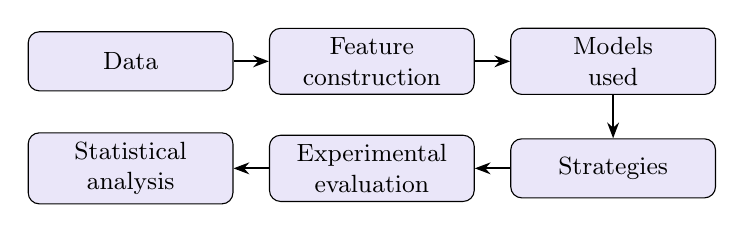
\begin{tikzpicture}[
  node distance=0.55cm and 0.45cm,
  pipebox/.style={draw, rounded corners, fill=blue!10, minimum width=2.6cm, minimum height=0.75cm, align=center, font=\footnotesize},
  arrow/.style={-{Stealth[length=2mm]}, thick}
]
\node[pipebox] (data) {Data};
\node[pipebox, right=of data] (features) {Feature\\construction};
\node[pipebox, right=of features] (models) {Models\\used};
\node[pipebox, below=of models] (strategies) {Strategies};
\node[pipebox, left=of strategies] (evaluation) {Experimental\\evaluation};
\node[pipebox, left=of evaluation] (stats) {Statistical\\analysis};

\draw[arrow] (data) -- (features);
\draw[arrow] (features) -- (models);
\draw[arrow] (models) -- (strategies);
\draw[arrow] (strategies) -- (evaluation);
\draw[arrow] (evaluation) -- (stats);
\end{tikzpicture}
\caption{Pipeline effectively executed in the experiments reported in Chapter~\ref{cap:experimental-evaluation}.}
\label{fig:executed-pipeline}
\end{figure}


\section{Research Design and Positioning} \label{sec:positioning} \label{sec:research-design}

The study compares two strategy variants on a common market window, execution model and set of price-derived inputs. The \emph{baseline} uses price-derived features only; the \emph{hybrid} adds a news-derived feature family. The question of Section~\ref{sec:objectives} is whether that addition improves risk-adjusted, cost-adjusted return. The comparison is a paired historical simulation, not a randomized intervention, and it does not assert a causal mechanism by which news moves exchange rates. Table~\ref{tab:variables} lists the variables by role.

\begin{table}[htbp]
\centering
\caption{Experimental variables of the present work.}
\label{tab:variables}
\small
\begin{tabular}{p{3.0cm}p{9.8cm}}
\toprule
\textbf{Role} & \textbf{Variables} \\
\midrule
Independent (manipulated) &
Presence or absence of the news feature family (baseline versus hybrid); in the follow-up studies, the entry rule, the exit horizon and the retraining policy. \\
\midrule
Dependent (measured) &
Net return and equity curve after costs, maximum drawdown, number of trades, hit rate and payoff ratio; prediction quality (log-loss, directional accuracy) where a model is evaluated on its own. \\
\midrule
Controlled (fixed) &
Instrument (EUR/USD), execution model and costs, starting deposit, model family, random seed, feature definitions, and the frozen model artifacts and their hashes. \\
\bottomrule
\end{tabular}
\end{table}

The closest published work is that of \citeonline{zhang2025macroalpha} (Section~\ref{sec:hybrid}), which reports cost-adjusted Sharpe ratios of 5.87 on EUR/USD and 4.65 on USD/JPY under five-fold expanding-window cross-validation on daily features. The present work differs in four respects that matter for any comparison of numbers. It trades at minute resolution rather than daily; it uses GDELT \emph{event} intensity rather than article sentiment; it passes the model output through a deterministic rule chain with a per-decision audit trail instead of a single threshold; and it evaluates on chronological splits with a replayed execution engine rather than on cross-validation folds. The numerical results are therefore not directly comparable, and Chapter~\ref{cap:experimental-evaluation} discusses the comparison on that basis.

\section{Data} \label{sec:data-architecture}

\textbf{Prices.} The price series is EUR/USD tick data from the Dukascopy public historical datafeed\footnote{\url{https://www.dukascopy.com/}}. Ticks are decoded, stored as Apache Parquet, and resampled to one-minute bid/ask bars (\texttt{QuoteBar}) with a tick count. A single venue is used throughout, so that all backtest prices come from one quote stream. USD/JPY was part of the original design but was not run in any reported experiment.

\textbf{Event data.} The news signal is built from GDELT 2.0 coded events \cite{leetaru2013gdelt}, materialized from the public BigQuery tables into daily Parquet partitions. GDELT collection for the target window starts on February 18, 2015, so March 2015 is the first fully covered month. A month enters an experiment only after its completion marker exists. Failed acquisition attempts and retry details are retained only as repository evidence.

\textbf{Why event intensity and not text sentiment.} The news input of the executed pipeline is the daily mean Goldstein score of coded events \cite{goldstein1992scale}, not a sentiment score inferred by a language model. The choice reflects both scope and validity. The Global Knowledge Graph carries extracted metadata (themes, entities, tone, quotations) and not the full text of articles\footnote{GDELT Global Knowledge Graph Codebook V2.1, \url{http://data.gdeltproject.org/documentation/GDELT-Global_Knowledge_Graph_Codebook-V2.1.pdf}.}, and materializing it for the whole window was out of reach within the available time and budget. In addition, the Goldstein mapping is a fixed, published scale, so the feature does not depend on a trained model whose training data would have to be checked against the evaluation years. The index is also a deterministic aggregate of a public table, which keeps every run recomputable. The cost is that the text half of the news family stays empty in all reported runs. Whether article text would add information remains open.

\textbf{Chronological allocation.} Each experiment fixes three non-overlapping spans: a family-fitting span for the LightGBM models, a later calibration span for the logistic combiner, and a held-out simulation span replayed by the engine with frozen models. Rows whose forward label horizon crosses a span boundary are purged. The pilot uses February--June 2015 for fitting, July for calibration and September for simulation; the main protocol uses March--December 2015, January 2016 and March--October 2016 (Section~\ref{subsec:one-year-protocol} of Chapter~\ref{cap:experimental-evaluation}). Observation counts are minute rows with overlapping labels and are not independent replications.

\section{Feature Construction} \label{sec:feature-layer}

Features are computed with strict point-in-time discipline: at time $t$, only data with timestamp $\leq t$ enter a feature, indicators are warmed up before any decision, and the training and engine code paths share one feature-definition function. Three price-derived families and one news-derived family are used.

\subsection{Trend features} \label{subsec:ta-structural-features}

The trend family classifies the market direction from exponential moving averages of the minute close (periods 3, 8 and 60) and reads the direction on a higher timeframe through Heikin-Ashi bars \cite{valcu2004heikinashi}. The same perception drives the trend-regime filter F1, which vetoes a decision when the primary and higher-timeframe directions conflict.

\subsection{Indicator features} \label{subsec:indicator-features}

The indicator family contains standard momentum and volatility measures \cite{murphy1999technical}: moving averages, MACD, RSI and ATR. Periods are fixed before any backtest, so that hyperparameter search does not silently extend over the indicator family.

\subsection{Candlestick-pattern features} \label{subsec:pattern-features}

The pattern family encodes candlestick shapes \cite{nison1991candlestick}. Detectors come from the TA-Lib library (\texttt{CDL*} functions)\footnote{\url{https://ta-lib.org/functions/}.} and are emitted only at the bar that closes the pattern. The first pilot used a simple placeholder detector; the TA-Lib detectors enter from the H4 experiments onward (Chapter~\ref{cap:experimental-evaluation}).

\subsection{Event-intensity features} \label{subsec:sentiment-features} \label{subsec:event-features}

The news family is the daily GDELT event intensity of the previous section. Because a daily aggregate is only knowable once its UTC day has ended, it is forward-filled onto the minute grid with a one-day publication lag: the aggregate of day $D$ is visible from 00:00~UTC of day $D+1$. A residual leak is recorded rather than hidden: the aggregate is keyed by the date on which an event occurred, not the date on which GDELT added the record, so an event reported more than one day late is folded into a day whose aggregate is already visible.

\section{Models Used} \label{sec:fusion}

\subsection{Late fusion: per-family models and a logistic combiner} \label{subsec:late-fusion}

One LightGBM classifier is fitted per feature family, using only the family's own features, to predict a fixed-horizon binary label: 1 if the mid price fifteen minute bars after the decision bar is strictly higher than at the decision bar, and 0 otherwise. The baseline has three family models (trend, indicator, pattern) and the hybrid adds a fourth (news).

The meta-learner is a logistic regression with default regularization. \textbf{Its inputs are exclusively the up-move probabilities produced by the family models}, one column per family (three for the baseline, four for the hybrid); raw features such as RSI, MACD or ATR never reach it. Its inputs are therefore on a common probability scale in $[0,1]$. The logistic regression is fitted on the calibration span, on the family models' out-of-sample predictions, so that the in-sample fit of the family models does not leak into the combiner. Its output $\hat{p}_t$ is the single probability read by the terminal filter. The baseline and the hybrid share this specification; the only difference is whether the news-family probability is a combiner input.

Fitted models are saved in a portable, pickle-free format with their provenance (split boundaries, label horizon, input hashes, code revision, library versions, seed 42), and every replay loads the same frozen artifacts and records their hashes.

\section{Strategies} \label{sec:strategies}

\subsection{Deterministic execution as a filter chain} \label{subsec:deterministic-execution}

A strategy turns $\hat{p}_t$ into a trade decision through a chain of deterministic \emph{filters} applied in sequence. Each filter contributes a recommendation and a reason and may veto, short-circuiting the chain to HOLD. Every decision is written to a bar-level decision table with the identifier of the trade it opened, managed or closed, so each trade can be traced to the contribution of every filter. The executed chain has seven filters: F1 trend regime, F2 indicator, F3 candlestick pattern, F4 news context (hybrid only), F5 risk guard (drawdown and exposure caps), F6 capital management (stop, targets, lot from risk) and F7, the terminal rule
\begin{equation*}
\mathrm{decision}_t = \begin{cases}
\text{BUY}  & \text{if } \hat{p}_t > \theta_{\text{high}} \text{ and } v_t = 0 \text{ and } (\neg g \lor r_t = \text{bull}), \\
\text{SELL} & \text{if } \hat{p}_t < \theta_{\text{low}} \text{ and } v_t = 0 \text{ and } (\neg g \lor r_t = \text{bear}), \\
\text{HOLD} & \text{otherwise},
\end{cases}
\end{equation*}
where $r_t$ is the trend regime from F1, $v_t$ the event-veto flag from F4 and $g$ a regime-gate switch. The thresholds $\theta_{\text{high}}$ and $\theta_{\text{low}}$ are fixed in the strategy configuration (0.55 and 0.45 in the main protocol); the calibration span is used to check them and the grid is recorded, but they are not learned. Every filter parameter lives in a YAML descriptor rather than in code, so a variant differs from its base by a configuration diff, and the resolved configuration is saved with each run. The values used are tabulated in Chapter~\ref{cap:experimental-evaluation}.

The separation between a model-based perception layer and this rule-based execution layer is the central design commitment (\emph{agentic perception, deterministic execution}). Model outputs are computed once and read at backtest time, so given the same features and thresholds a replay is reproducible regardless of upstream non-determinism.

\subsection{Strategy variants} \label{subsec:strategy-variants}

The experiments compare the following variants, all on the same chain and execution model. The \textbf{baseline} uses the three price-family models. The \textbf{hybrid} adds the news-family probability to the combiner and the F4 event gate; its comparison with the baseline therefore measures the combined effect of both, and isolating either requires a separate ablation. The follow-up studies add: rule-based news cells (event-intensity trigger on a trailing-quantile threshold, with reversed-sign and always-short controls); an H4/H1/M15 timeframe sweep with TA-Lib patterns and a quote-activity gate; a news-only strategy registered before its outcome; the frozen policy of the adaptive-retraining study; and a screen of a 22-pattern candlestick catalogue, per pattern, in combination and under gated variants. Their definitions and registration dates are summarized with their results in Chapter~\ref{cap:experimental-evaluation}; the full registry is kept in the repository.

\section{Experimental Evaluation} \label{sec:evaluation}

\subsection{Execution engine} \label{sec:execution-engine}

Backtests run on the open-source LEAN engine of QuantConnect, released under the Apache~2.0 license\footnote{\url{https://github.com/QuantConnect/Lean/blob/master/LICENSE}.}, executed locally in a Docker container with its Python algorithm interface. No QuantConnect cloud service is used. The Parquet price store is materialized once into LEAN's native format, and an automated test inside the pinned engine image confirms that training features and the engine's features agree to nine decimal places on every decision bar.

\subsection{Experimental workflow} \label{subsec:workflow-stages}

Each experiment is registered before its evaluation returns are inspected, with hypothesis, variants, label, dates, execution assumptions, primary comparison and candidate-search budget. Family models and combiner are fitted and frozen; the frozen artifacts are replayed over the held-out window under identical assumptions with no fitting in the replay; and the replay is audited (coverage, decision-to-trade joins, zero-trade outcomes) before any metric is read. A registered job is labelled \emph{registered}, \emph{exploratory} or \emph{ad hoc} according to whether its design was written down before any outcome of its window was read. A window that has guided later model or threshold choices becomes development data and is not presented as an untouched test set.

\subsection{Execution model and costs} \label{subsec:execution-assumptions}

The pilot sized orders as a fraction of equity and applied the 0.3-pip median spread of the quote bars. From the confirmation reruns onward the execution model of Section~\ref{subsec:execution-model} is used: stop-first sizing from a fixed risk fraction, one target and a trailing stop, a limit of two concurrent trades, and 1.0 pip of slippage per fill. Both variants inherit identical execution assumptions by construction. Known-answer controls on the engine check costs, sizing, stops, margin and leverage before any outcome is interpreted, because a successful container run does not establish economic realism.

\section{Statistical Analysis of Results} \label{sec:reproducibility}

\subsection{Rule-level significance under multiple comparisons} \label{subsec:rule-significance}

Cross-validation alone does not remove selection bias when many candidates are screened on the same history \cite{aronson2007evidence,bailey2017overfitting}, so the full search history, including unsuccessful variants, accompanies every inferential claim. Inference uses net daily portfolio returns taken from the engine's actual equity, including open-position valuation, at recorded UTC day boundaries; the analyzer neither interpolates missing equity nor substitutes closed-trade returns. The engine's annualized Sharpe ratio is descriptive.

For paired comparisons the estimand is the mean daily difference in net return, tested with the stationary bootstrap of \citeonline{politis1994stationary} on identical circular blocks for both strategies, with a primary and a sensitivity block length fixed before evaluation. In a registered simulation study the procedure passed its size bound only at long windows (twenty-day blocks at twelve hundred observations) and over-rejected at the ninety- and one-hundred-eighty-day windows (null rejection of 9\% to 14\% at the nominal 5\%). Short-window results are therefore diagnostic only, and a mean-return test does not establish Sharpe superiority.

The deflated Sharpe ratio of \citeonline{bailey2014deflated} is implemented from the non-annualized daily Sharpe ratio, skewness and kurtosis, with the selection threshold computed from across-trial Sharpe dispersion and a documented number of effective independent trials; missing selection history yields an unavailable result and not an assumed single trial. For rule cells, a drift control (always-short or always-long on the same bars) separates the effect of the signal from the effect of the currency's path. For pattern screening, a pooled multiple-comparisons check asks whether the best of the screened candidates is distinguishable from the chance outcome of screening that many (Section~\ref{subsec:candles-multiple-comparisons}). Classification-quality metrics are reported separately from, and are never taken as evidence of, trading profitability.

\subsection{Threats to validity} \label{subsec:threats-summary}

The threats are organized along the four biases of \citeonline{hallsmoore2015}. \emph{Optimization bias} is the dominant risk: repeated threshold, gate and strategy selection on the same months means that no reused window is confirmatory, and only windows that no earlier decision had read are treated as out-of-sample. \emph{Look-ahead bias} is addressed by the one-day event lag, the purging of labels at split boundaries, the feature-parity test, and decisions taken at bar close; the residual event-date leak above is disclosed. \emph{Survivorship bias} is not assessed separately, since the study uses one currency pair and not a selected universe of instruments. Registering experiments before viewing outcomes and reporting all variants run limits the room for selective reporting. \emph{Psychological tolerance bias} is not assessed, since the strategies were evaluated by replay and not operated live. The evaluation is a single pair over one year, with one chronological split per experiment, and cannot distinguish a weak regime-dependent edge from the particular year's price path.

\section{Scope: Designed but Not Executed} \label{sec:methodology-scope}

The original design contained more than was run. The following components were not exercised in any reported experiment and are not part of the evidence: additional corpora (FNSPID, CC-News, central-bank releases, Reddit, social-media streams); the dictionary and FinBERT-class sentiment scorers and the GPR index as model inputs; the market-activity feature family; USD/JPY; the extended filter catalogue (F8--F20); the search over filter order and per-filter timeframe; combinatorial purged cross-validation with embargo; rolling refits over a ten-year window; and the four adaptive-retraining policies other than the frozen one. They are developed as future work in Section~\ref{subsec:future-unexecuted} of Chapter~\ref{cap:conclusion}.

\chapter{Experimental Evaluation} \label{cap:experimental-evaluation}

This chapter distinguishes implemented tooling, exploratory execution, and evidence that could support the research hypothesis. The predecessor snapshot is September 28, 2026, at 00:36 UTC (September 27 in the operator's Pacific timezone); Section~\ref{subsec:h4-snapshot} adds the completed H4 matrix at 01:11 UTC without replacing that historical record. The workflow in Section~\ref{subsec:workflow-stages} governs the transition between these states. A completed training job or a successful engine replay does not by itself constitute a validated comparison.

\section{Experimental Setup} \label{sec:experimental-setup}

The price-download and transformation path, event-feature construction, offline F7 trainers, baseline and hybrid LEAN strategies, decision audit, and analysis commands are implemented. Their existence does not imply that every proposed source or experiment has run. The present pilot uses EUR/USD minute prices and GDELT event intensity. Text sentiment, a real F3 pattern detector, and the proposed broader feature set are absent from this pilot. It must therefore be described as an event-augmented comparison, not as a completed NLP-sentiment study.

The first six available months are allocated to fitting and calibration as shown in Table~\ref{tab:pilot-splits}. The family models use February--June, and logistic stacking uses July. July is not a held-out test for the combined model. The existing trainer also constructs an August test partition, which is excluded from fitting. The initial requested simulation window is September. The start date of February 2 follows from the event feature's one-day publication lag.

\begin{table}[htbp]
\centering
\caption{Chronological allocation for the fixed-model EUR/USD pilot.}
\label{tab:pilot-splits}
\small
\begin{tabular}{p{4.0cm}p{4.0cm}p{5.0cm}}
\toprule
\textbf{Stage} & \textbf{Inclusive dates} & \textbf{Role} \\
\midrule
Family fitting & February 2--June 30, 2015 & LightGBM parameters \\
Combiner calibration & July 1--31, 2015 & Logistic stacking parameters \\
Trainer held-out partition & August 1--31, 2015 & No fitting; not a replay result \\
Initial simulation & September 1--30, 2015 & Frozen-model engine replay \\
\bottomrule
\end{tabular}
\end{table}

Both offline training jobs completed and saved separate portable model artifacts. Each log records 153,531 fitting rows, 32,813 calibration rows, and 30,297 held-out rows, for 216,671 rows in total. These are observation counts, not independent replications. Labels use a fifteen-minute midpoint direction and are purged at split boundaries. The current setup is a single chronological fit, not rolling retraining or CPCV. Additional held-out months can reuse these frozen models; a refit must be registered separately.

In the initial historical pilot, the baseline September replay completed with zero closed trades. Its recorded identifier is \path{baseline/20260927T044836-4cd12c922200}; the UTC identifier falls on September 27 although execution occurred on September 26 in the operator's Pacific timezone. A zero-trade replay requires investigation of coverage, model outputs, and filter vetoes before interpretation. Its zero return and zero-valued summary statistics are not evidence of strategy efficacy or a validated null result. The hybrid replay subsequently completed as \path{hybrid/20260927T053156-4f2ebf081eaf}, also with zero closed trades. Both saved engine files contain the daily equity endpoints for September. Their flat equity cannot estimate return variance or paired uncertainty; the integration check must report unavailable statistics. No paired performance or significance result is claimed here.

Artifacts are kept in the directory \path{2026-09-26-six-month-pilot/} beneath the local \path{algo-suite/data/training/} root. Model JSON files contain split metadata, input hashes, configuration, code revision, and package versions. The job records stage logs and exit status; run directories contain \path{run.json}, \path{trades.json}, \path{metrics.json}, \path{strategy-config.json}, LEAN outputs, and the chain's \path{decisions.parquet}. The repository progress record tracks the initial missing-broker-configuration failure and the resumed OANDA run. These local artifacts must be archived with the final report; a documentation snapshot is not a substitute for them.

The remaining gates are coverage reconciliation for the BigQuery materialization path, point-in-time event availability, execution-cost and risk-economics review, known-answer engine controls, and inspection of decision/trade evidence. Story 11 delivered the corrected inference software of Section~\ref{subsec:rule-significance}; each empirical use of it still requires audited daily equity, cost metadata, actual selection history and block settings registered before evaluation. The wider validation study, additional pairs, and feature ablations remain separate work. The following results are descriptive intermediate observations; unfinished stages remain explicitly unavailable.

\subsection{Snapshot provenance and effective parameters} \label{subsec:intermediate-provenance}

The evidence archive is located beneath the repository root at:
\begin{quote}
\small\ttfamily
algo-suite/docs/stories/in-progress/\\
13-pattern-volume-experiments/evidence/
\end{quote}
The file \path{snapshot-20260928T003601Z.json} records source paths, SHA-256 hashes, code and model identities, job scripts, log excerpts, manifests, and configuration artifacts. The companion \path{per-run-parameters-20260928T003601Z.md} joins each reference R01--R20 to its full run identifier, result, F1--F7 parameter matrix, and per-field provenance. References in the tables and figure legends use these same keys. The clock was confirmed at 00:36:01 UTC; the read-only collection ended at 00:36:02 UTC. It is a bounded snapshot of active jobs, not a claim about their eventual outcomes.

Sixteen run manifests record \path{success=true}; four further runs have live processes but no final manifest. No inspected final manifest records failure. A separate historical failed launch reports a missing \path{broker.adapter}; its result and effective parameters are unavailable. The execution-realism job has completed September and October for both strategies, is running the November baseline, and has not yet started the November hybrid. The A05 sweep has four completed variants and one running variant; the four SpockFX-derived variants have completed. Both annual-protocol simulations are still running. The parallel scripts use bare \path{wait}, so a parent exit code of zero does not establish success of every child; completion here requires each run's own manifest.

The execution-realism and sweep jobs record revision \path{7165308778fd}. Their frozen pilot model hashes begin \path{1a6fd37e96de} (baseline) and \path{a6dda4c2effc} (hybrid). Full revision identifiers, hashes, and training provenance are in the archive. The earlier ungated job records revision \path{709b9bd4bdcf} with uncommitted changes; the pilot hybrid training provenance also carries a dirty revision. Those commit identifiers alone cannot reconstruct the missing patches.

\begin{table}[htbp]
\centering
\caption{Compact parameter reading for execution-model runs R08/R09 (baseline) and R13/R14 (hybrid). The full per-run matrix, including missing historical fields, is in the evidence appendix.}
\label{tab:intermediate-filter-parameters}
\small
\begin{tabular}{p{1.1cm}p{12.2cm}}
\toprule
\textbf{Filter} & \textbf{Archived settings and evidence limits} \\
\midrule
F1 & EMA perception recorded in runtime logs; upstream EMA periods 3/8/60 on minute bars. The 60-period EMA is not an H1/H4 bar series. \\
F2 & RSI period 14, midline 50; MACD 12/26/9, histogram threshold 0. \\
F3 & Bullish: engulfing, hammer, morning star; bearish: engulfing, evening star, shooting star. These configured names do not imply a detector: the predecessor runtime supplies no candle pattern. \\
F4 & Absent from baseline; hybrid event-intensity veto threshold $-0.5$ and sentiment-direction threshold 0.15. Text sentiment is absent in these runs. \\
F5 & Daily/weekly drawdown limits $-0.05/-0.15$; concurrent-trade cap 2; portfolio-at-risk cap 0.10. Configured limits are not independently verified enforcement. \\
F6 & Risk fraction 0.03; swing lookback 60 bars; stop shrink 0.20; minimum 5 pips; minimum reward/risk 2. Target: 2R closes 0.5; trailing step: at 0.5R, stop to $-0.66$R. \\
F7 & Thresholds 0.55/0.45; regime gate off; label horizon 15 minutes. Families: trend, indicator, pattern; hybrid additionally includes news. \\
\bottomrule
\end{tabular}
\end{table}

The same four runs record starting cash 10,000 and shared execution settings: spread 1 pip, commission per lot 0, broker stop level 0, minimum holding bars 0, and \path{close_on_veto=false}. These are archived assumptions, not an economic validation. All fourteen available JSON/YAML configuration pairs agree. The initial and ungated runs R06/R07/R11/R12 lack archived YAML and parameter provenance, and their JSON omits several filter settings; those values remain \textit{missing}, without substitution from current defaults. Running R10 and R19 also lack their own configuration JSON/YAML at this snapshot. A provenance file naming a source is not a substitute for its missing effective values.

\subsection{Annual protocol: training diagnostics and unfinished replay} \label{subsec:intermediate-annual}

The annual job fits family models on March 2--December 31, 2015, calibrates the combiner on January 2016, and constructs a February 2016 held-out partition. Both saved models record 312,878 fitting, 28,802 calibration, and 30,120 held-out rows. Their SHA-256 prefixes are \path{0b41fd39ebf3} and \path{b67ac32e1fc5}; their recorded training revision is the Story 12 revision above. The planned continuous replay spans March 1--October 31, 2016. Baseline R19 and hybrid R20 have no final \path{run.json} or \path{metrics.json}; no annual return is reported. Their full run identifiers and launched arguments are preserved in the appendix.

The saved threshold grid shows descriptive anti-alignment between F7's upward-direction probability and the trend regime. In January, baseline mean probabilities are 0.4791 in bull regimes and 0.5149 in bear regimes; hybrid values are 0.4794 and 0.5148. At thresholds 0.55/0.45, enabling the regime gate leaves only two sell signals for either model, whereas disabling it yields 1,242 baseline and 1,125 hybrid signals. The corresponding ungated label hit rates are 0.569 and 0.564. These are calibration diagnostics over overlapping fifteen-minute labels, not realized trade win rates, independent trials, or proof of profitable anti-trend trading. They do not identify the cause of the replay losses.

The calibration script actually inspects both January and February, including the nominal held-out partition, across eight threshold pairs and both gate settings for each model (64 recorded combinations across the two spans). Thus February is held out from fitting but has already been inspected diagnostically. An untouched-2016-data claim would be false. Any later choice informed by these grids or the ongoing replay must enter the selection history; this snapshot establishes no confirmatory result.

\section{Data Coverage} \label{sec:coverage-results}

\textit{To be added in the final version.}

\section{Baseline Strategy} \label{sec:baseline-results}

The ungated September development replay R07 records 1,032 closed trades and a return of $-0.05\%$ with \path{size=0.5} and \path{cash=10000}. The later execution-model runs use a different sizing and exit contract and record much larger losses (Table~\ref{tab:intermediate-replays}). These are separate experiments on reused historical data; their difference cannot isolate a single execution parameter's effect. The November baseline R10 is still running at the snapshot.

\begin{table}[htbp]
\centering
\caption{Completed execution-model replays, with their own effective parameters linked by R reference to Table~\ref{tab:intermediate-filter-parameters} and the full evidence appendix. Returns and maximum drawdowns are copied from \texttt{metrics.json}; trade counts are from successful \texttt{run.json} manifests.}
\label{tab:intermediate-replays}
\small
\begin{tabular}{llrrr}
\toprule
\textbf{Ref./strategy} & \textbf{Month} & \textbf{Closed trades} & \textbf{Return (\%)} & \textbf{Max DD (\%)} \\
\midrule
R08 baseline & Sept.\ 2015 & 320 & $-52.57$ & 53.8 \\
R13 hybrid   & Sept.\ 2015 & 322 & $-52.75$ & 54.0 \\
R09 baseline & Oct.\ 2015  & 319 & $-53.35$ & 55.2 \\
R14 hybrid   & Oct.\ 2015  & 349 & $-51.37$ & 53.3 \\
\bottomrule
\end{tabular}
\end{table}

The appendix joins each result (R08, R13, R09, R14) to its full run identifier, manifest hash, and model hash. Each month starts separately from 10,000; the months are not presented as a single continuously funded account.

\section{Hybrid Strategy} \label{sec:hybrid-results}

The ungated September development replay R12 records 1,069 closed trades and $+0.51\%$ return under the earlier execution contract. Under the later contract, both completed hybrid replays lose more than half the starting account value, as Table~\ref{tab:intermediate-replays} shows. The baseline--hybrid ordering changes between September and October. Neither ordering supports a news-effect claim without paired inference, audited costs, and the full exploratory selection history.

\begin{figure}[htbp]
\centering
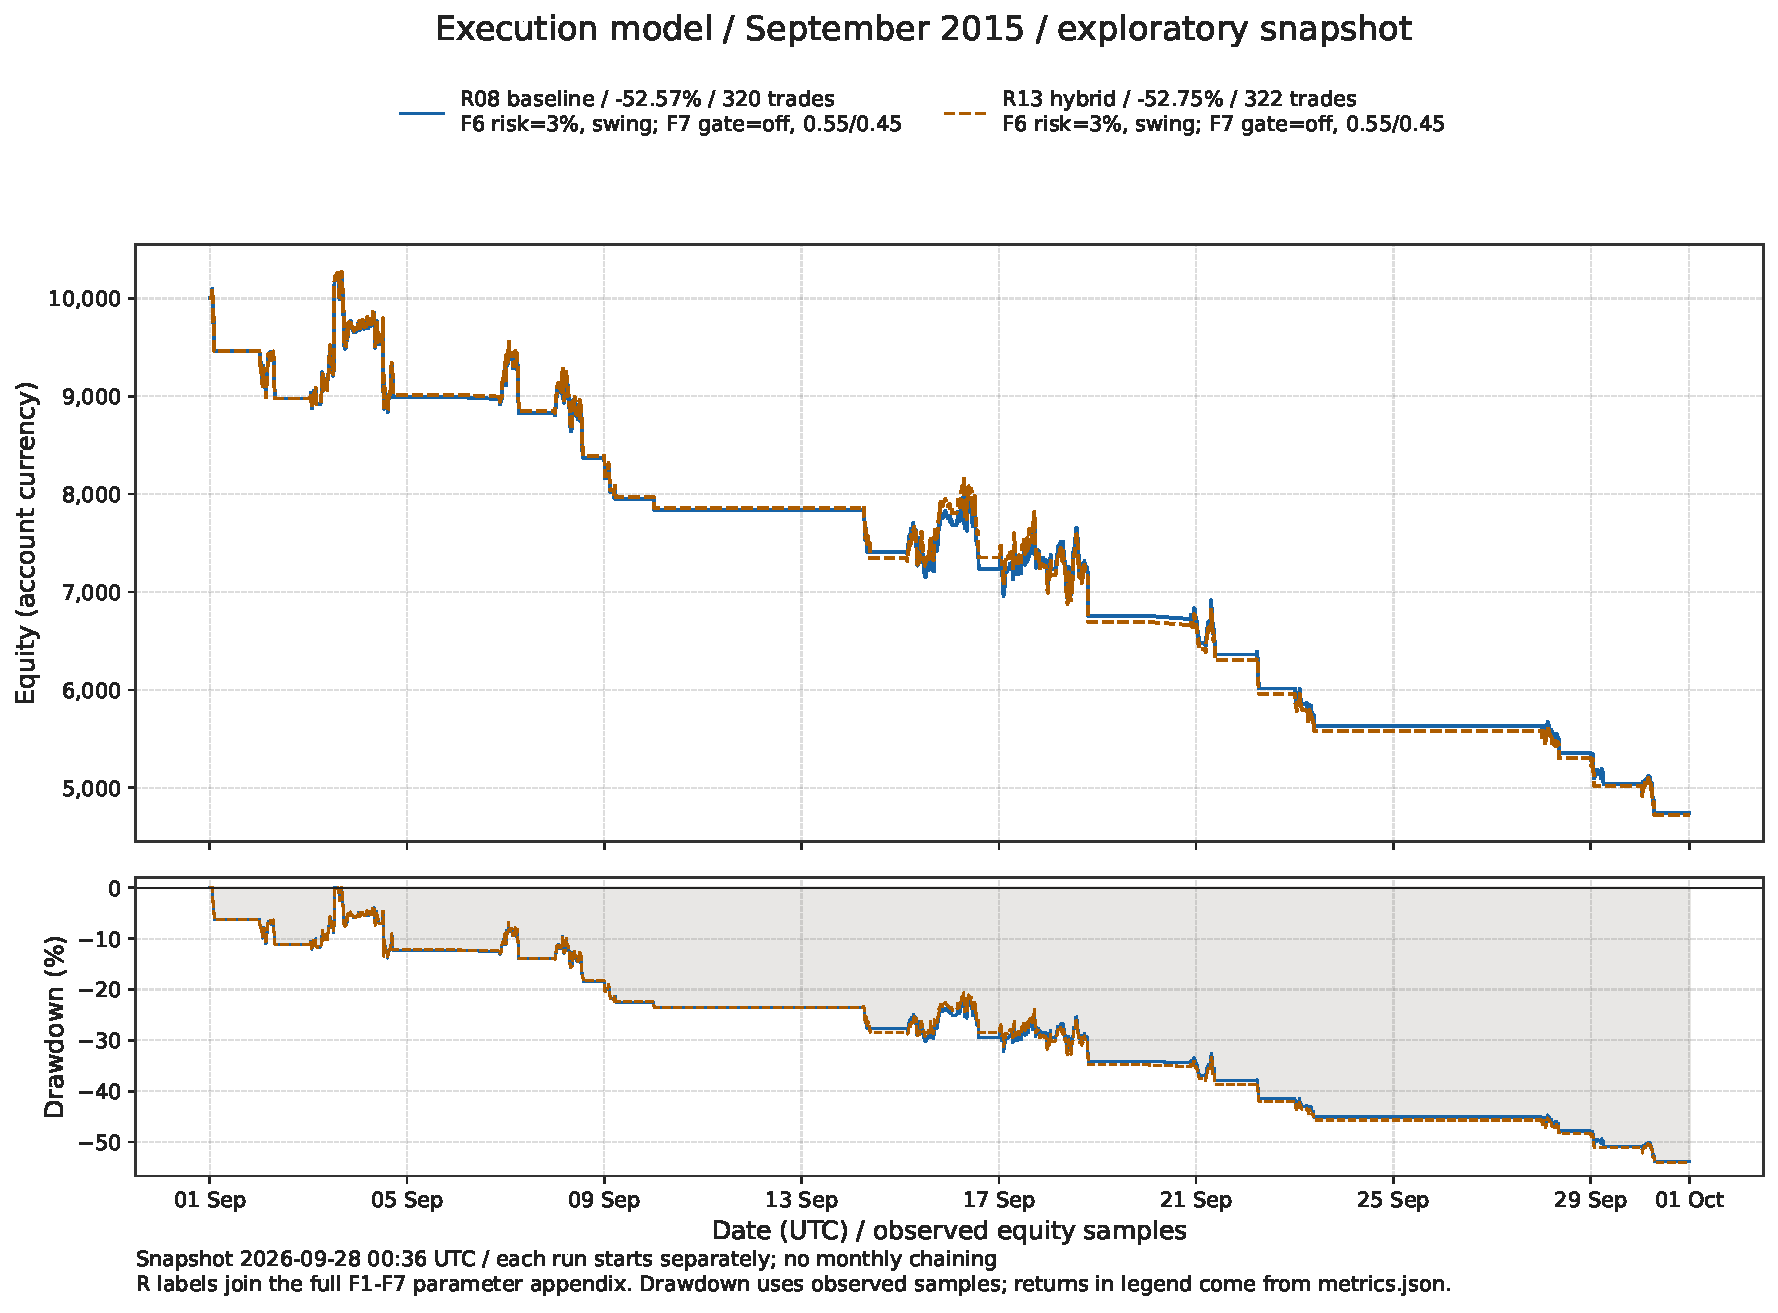
\includegraphics[width=\textwidth]{../algo-suite/docs/stories/in-progress/13-pattern-volume-experiments/evidence/figures/execution-september-print.pdf}
\caption{Observed September equity and drawdown for completed runs R08 and R13, in 2:1 panels. Legends join the parameter appendix; curves use the original \texttt{equity.csv} samples. Drawdown is relative to each sampled running peak and need not equal the engine's rounded maximum-drawdown statistic.}
\label{fig:intermediate-equity}
\end{figure}

Figure~\ref{fig:intermediate-equity} and the October and sweep figures in the evidence archive reuse the repository's equity reader and drawdown calculation. Their presentation adapts the \textit{trading-visualization} skill's Matplotlib layout and styling guidance\footnote{\url{https://github.com/agiprolabs/claude-trading-skills/tree/main/skills/trading-visualization}}; that software guidance supplies no empirical performance evidence. Dark PNG and print PDF variants are provided. No synthetic curve, monthly rebasing, or unfinished annual result is plotted.

\section{Ablations} \label{sec:ablations}

The September sweeps are exploratory parameter comparisons using the frozen pilot baseline model. Table~\ref{tab:intermediate-sweeps} retains losing and zero-trade variants. R02 (a05-gated) remains running with no final result. The full F1--F7 configuration of every listed run, including parameters not varied, is joined to its R reference in the appendix.

\begin{table}[htbp]
\centering
\caption{Completed September-2015 exploratory variants. Every row links its result to its own archived filter matrix by R reference; zero trades do not establish robustness.}
\label{tab:intermediate-sweeps}
\small
\begin{tabular}{llrrr}
\toprule
\textbf{Ref.} & \textbf{Variant} & \textbf{Closed trades} & \textbf{Return (\%)} & \textbf{Max DD (\%)} \\
\midrule
R01 & a05-conservative & 3 & $-0.81$ & 10.8 \\
R03 & a05-risk1 & 552 & $-55.28$ & 55.4 \\
R04 & a05-selective & 6 & $-3.76$ & 5.6 \\
R05 & a05-wide-stop & 14 & $-17.65$ & 21.5 \\
R15 & spockfx-dragon03 & 144 & $-53.47$ & 55.8 \\
R16 & spockfx-dragon03-atr & 437 & $-42.16$ & 50.1 \\
R17 & spockfx-dragon05 & 0 & 0.00 & 0.0 \\
R18 & spockfx-setupnow & 0 & 0.00 & 0.0 \\
\bottomrule
\end{tabular}
\end{table}

The SpockFX labels describe selected plan adaptations, not faithful replications of the reference strategies. At reference revision \path{a1ed6b43b3a7}, \path{deploy.xml} declares a 60-minute selector with a 20\% stop cut and 240-minute deployment templates with a 50\% cut. These H1/H4 settings, indicator-based entry/stop buffers, and strategy rules are not equivalent to the M1 EMA chain and frozen model used in these sweeps. For example, R16 actually archives ATR multiplier 4, stop shrink 0.5, minimum stop 10 pips, and risk fraction 0.01; the YAML comment's ``2 x ATR14'' is not the configured pre-shrink multiplier. Increasing an M1 ATR multiplier does not create H4 candles. Results therefore cannot establish the performance of the original SpockFX system or of the new Story 13 candle/quote-activity implementation.

\subsection{Completed H4 candle and quote-activity matrix} \label{subsec:h4-snapshot}

The second snapshot, clock-confirmed at September 28, 2026, 01:11:14 UTC, contains all four baseline-v1 and four hybrid-v2 Dragon08 H4 swing-proxy cells. Both parent processes record exit 0, both final input checks pass with no errors or mismatches, and all eight individual manifests record success. The interrupted hybrid-v1 root is retained separately: its first two cells succeeded, but its last two logs report ENOSPC before creating their result directories. Its controller-observed parent exit was 1 and its final integrity report is missing. It is not a completed matrix or an additional replication.

The H4 archive joins H01--H08 to each cell's full configuration JSON/YAML, field provenance, model SHA-256, training revision, result manifest, trades, equity, and source fingerprints. Its files, beneath the evidence directory given above, are:
\begin{quote}
\small\ttfamily
h4-snapshot-20260928T011114Z.json\\
h4-parameters-20260928T011114Z.md
\end{quote}
All eight runtime configurations match their prepared JSON, YAML, and model training configuration. The two matrix manifests have identical maps of 249 code-file hashes, despite different recorded Git revisions during concurrent documentation commits. These source fingerprints, not a commit identifier alone, establish the recorded implementation identity.

\begin{table}[htbp]
\centering
\caption{All completed exploratory September-2015 H4 cells. H references join the full per-cell parameter/model appendix; no cell is omitted. Maximum drawdown is the engine-reported statistic.}
\label{tab:h4-results}
\small
\begin{tabular}{lllcrrr}
\toprule
\textbf{Ref.} & \textbf{Family} & \textbf{F3} & \textbf{Volume} & \textbf{Trades} & \textbf{Return (\%)} & \textbf{DD (\%)} \\
\midrule
H01 & Baseline & Disabled & Off & 6 & 1.36 & 5.1 \\
H02 & Baseline & Disabled & On & 3 & 2.87 & 5.1 \\
H03 & Baseline & TA-Lib & Off & 6 & 1.36 & 5.1 \\
H04 & Baseline & TA-Lib & On & 3 & 2.87 & 5.1 \\
H05 & Hybrid & Disabled & Off & 6 & 1.36 & 5.1 \\
H06 & Hybrid & Disabled & On & 3 & 2.87 & 5.1 \\
H07 & Hybrid & TA-Lib & Off & 6 & 1.36 & 5.1 \\
H08 & Hybrid & TA-Lib & On & 3 & 2.87 & 5.1 \\
\bottomrule
\end{tabular}
\end{table}

Closed-trade counts come from both the manifest and the actual trade ledger, not from the reciprocal of a rounded win rate. No new cell has zero closed trades; earlier zero-trade and losing runs remain in the predecessor tables. Equity returns include open-position valuation at the endpoint and are not equivalent to realized closed-trade profit. Identical return rows are not independent replications. Within each volume setting, all four equity CSVs are byte-identical.

\begin{table}[htbp]
\centering
\caption{Effective H4 settings for H01--H08. Every filter is included; the H-keyed appendix repeats the complete resolved matrix and model identity alongside each result.}
\label{tab:h4-parameters}
\small
\begin{tabular}{p{1.2cm}p{12.1cm}}
\toprule
\textbf{Filter} & \textbf{Recorded settings} \\
\midrule
F1 & EMA perception; complete 240-minute bars; EMA 3/8/60. The 60-period series is an H4 EMA, not the reference H1 selector. \\
F2 & RSI 14 with midline 50; MACD 12/26/9 with histogram threshold 0; ATR period 14. \\
F3 & Disabled or TA-Lib per row. Bullish: engulfing, hammer, morning star; bearish: engulfing, evening star, shooting star. \\
F4 & Absent in H01--H04; H05--H08: event veto threshold $-0.5$, sentiment-direction threshold 0.15. Text sentiment is missing. \\
Volume & Absent in odd-numbered H rows; even rows use quote-tick activity, lookback 20 prior closed bars, minimum relative activity 1.0. Not exchange-traded volume. \\
F5 & Daily/weekly drawdown limits $-0.05/-0.15$; concurrent-trade cap 2; portfolio-at-risk cap 0.18. \\
F6 & Risk fraction 0.03; swing lookback 60; stop shrink 0.5; minimum 5 pips; minimum reward/risk 2. Targets 4R/6R, each closes 0.5; trail at 2R to $+0.1$R. \\
F7 & Separate model per cell; horizon 240 minutes; thresholds 0.55/0.45; regime gate off. Trend, indicator, pattern families; hybrid adds news. \\
\bottomrule
\end{tabular}
\end{table}

All cells start with cash 10,000 and record spread 1 pip, commission per lot 0, broker stop level 0, minimum holding bars 0, and \path{close_on_veto=false}. The H4 bar construction and Dragon08 exit settings distinguish these cells from the earlier M1 sweeps, but reference SpockFX entry, stop, trend-buffer, and exit semantics remain replaced by research proxies. Neither faithful replication nor economic validity follows from these settings.

The effective sample is especially small: the controller's completed-bar audit counts 110 September H4 bars, of which the first 59 are consumed by warm-up. Independently inspected decision artifacts contain only 51 decisions per cell, from September 16 at 20:00 UTC through September 30 at 20:00 UTC. Model provenance records 475 fitting, 114 calibration, and 214 test rows; the last count covers August--September and must not be presented as 214 September trading decisions.

\begin{table}[htbp]
\centering
\caption{Decision-level diagnostics, identical across the two families for the counts shown. F4 applies only to hybrid cells.}
\label{tab:h4-diagnostics}
\small
\begin{tabular}{p{8.4cm}rr}
\toprule
\textbf{Observation per cell} & \textbf{Volume off} & \textbf{Volume on} \\
\midrule
Audited decisions / F1 vetoes & 51 / 11 & 51 / 11 \\
Decisions reaching F3 & 40 & 40 \\
Disabled F3: abstentions & 40 & 40 \\
TA-Lib F3: abstentions / buys / sells & 32 / 4 / 4 & 32 / 4 / 4 \\
Hybrid F4: reached / vetoes & 40 / 0 & 40 / 0 \\
Quote-activity vetoes & 0 & 17 \\
Final SELL decisions / closed trades & 40 / 6 & 23 / 3 \\
\bottomrule
\end{tabular}
\end{table}

TA-Lib is not disconnected: F3 records four bearish engulfings, three bullish engulfings, and one hammer among the 40 reached decisions. Baseline F7 probabilities range from 0.408089--0.428667 with detection disabled and 0.408195--0.428762 with TA-Lib. Hybrid ranges are 0.389898--0.436169 and 0.389917--0.436204, respectively. All remain below the fixed SELL threshold 0.45. Pattern and event features change model probabilities without crossing a decision boundary in this sample; identical outcomes therefore do not demonstrate that patterns or news are generally useless. Hybrid F4 records 40 abstentions and no vetoes per cell. The controller's canonical-input audit reports event intensity 0.643298--0.903367, above the $-0.5$ veto threshold, and missing sentiment on all 40 reached decisions; its detailed diagnostic attribution is retained in the evidence synopsis.

\begin{figure}[htbp]
\centering
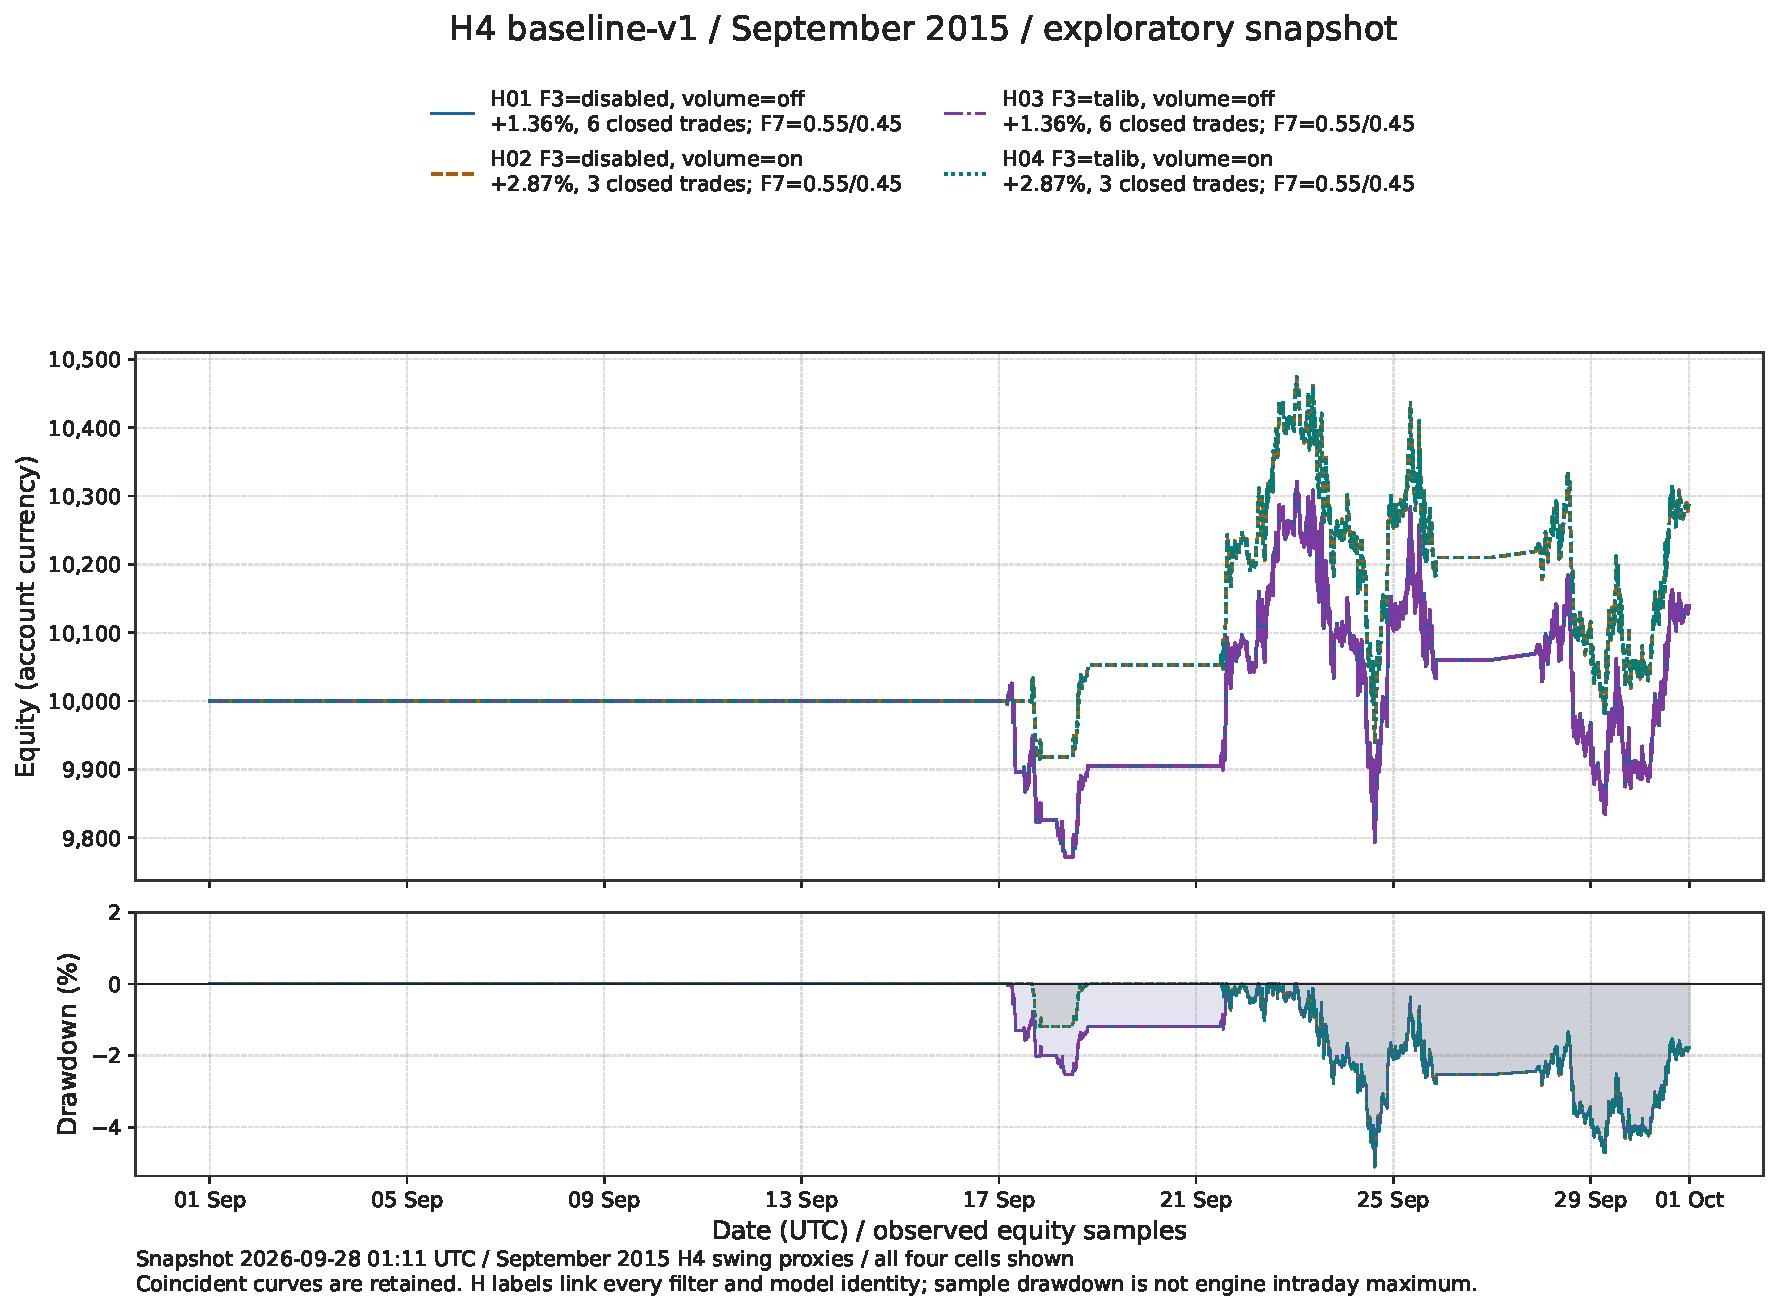
\includegraphics[width=\textwidth]{../algo-suite/docs/stories/in-progress/13-pattern-volume-experiments/evidence/figures/h4-baseline-v1-20260928T011114Z-print.pdf}
\caption{All four baseline H4 cells, including coincident curves. The archive also contains the four hybrid cells and dark-screen variants. Panels use actual equity samples and their drawdown in a 2:1 layout; sampled drawdown need not equal the engine's intraday maximum. Labels join the full parameter appendix.}
\label{fig:h4-equity}
\end{figure}

These favorable H4 observations do not supersede the predecessor losses or calibration anti-alignment. The reused September window, eight separate fitted models, multiple earlier exploratory selections, warm-up truncation, and only three or six closed trades prevent a confirmatory out-of-sample claim. No corrected significance, generalization, causal feature benefit, or economically validated strategy is established.

\section{Comparison with Closest Prior Art} \label{sec:zhang-comparison}

\textit{To be added in the final version.}

\section{Threats to Validity Specific to the Observed Results} \label{sec:experimental-threats}

The present evidence supports an implementation and execution report. It does not establish H1. A short single-pair window, overlapping labels, and daily event values repeated across minute rows limit generalization and invalidate treating row count as an independent sample size. Text sentiment is missing throughout; pattern detection is absent from the predecessor pilot but is observed in the new TA-Lib H4 cells.

Repeated inspection of September, gate changes, threshold grids, execution changes, and nine named sweep variants create multiple exploratory selection opportunities. Selecting the least negative or zero-trade run would not turn this development window into an out-of-sample confirmatory test. The observed losses and F7/regime anti-alignment must be retained alongside favorable historical numbers. The full search history, rather than only the two finally reported strategies, is required for any selection adjustment; the 64 grid entries alone are not an established effective trial count for DSR. Recorded configuration values do not prove effective enforcement, and a successful manifest does not close this economic-validation gap.

The hybrid introduces both a news-family model and an event gate, so a paired difference would represent their combined effect rather than an isolated sentiment contribution. The next-day event lag does not remove the documented late-reporting leakage from aggregation by event date. Fixed stop, pip-value, margin, and risk proxies require economic validation. Finally, schema-v2 inference in Section~\ref{subsec:rule-significance} requires complete daily equity, documented cost treatment and actual selection history. Legacy DSR adjustments and pooled-trade permutation outputs remain exploratory. An unavailable corrected statistic cannot be replaced with a legacy value. Subsequent runs must update this assessment with actual coverage, trade activity, cost assumptions, and paired uncertainty.

\chapter{Conclusion} \label{cap:conclusion}

\section{Final Remarks} \label{sec:final-remarks}

This work built a deterministic Forex evaluation pipeline that combines price-derived and news-derived features, then used it to test whether adding a news family to a price-only strategy improves cost-adjusted return. The executed study is a fixed-model EUR/USD evaluation: one baseline and one hybrid strategy replayed on LEAN under a common execution model, followed by registered follow-ups over one trading year (Chapter~\ref{cap:experimental-evaluation}). The ten-year, two-pair, multi-source design with rolling retraining and combinatorial cross-validation remains a target and not a result; it is mentioned in Section~\ref{subsec:future-unexecuted}.

\subsection{Answer to the research question} \label{subsec:answer-rq}

In the configuration tested, the hybrid strategy did not outperform the baseline, and no strategy variant showed an edge. Both March--October 2016 simulations on frozen models lose about 88\% of the deposit, and the news family changes the outcome by about \$65 over 1{,}029 trades. Fifty-one further tuning variants on the H4, H1 and M15 clocks confirm this: none is profitable in November 2016, the one month that no earlier decision had read, and the loss grows with the number of trades. Hypothesis~H1 is therefore not supported. The result is bounded by its scope: one currency pair, one year, a daily event-intensity index rather than article text, and a single chronological split per experiment. It does not show that news has no value for Forex prediction in general.

\subsection{Scientific findings} \label{subsec:scientific-findings}

The experiments yield six findings about method and signal, independent of the software that produced them.

\begin{enumerate}
    \item \textbf{A positive return does not imply predictive ability.} The single positive cell, the reversed-sign news rule at $+12.2\,\%$, is the euro's decline with leverage: its always-short control is statistically the same account ($p = 0.92$), and its long-side mirror loses $48.5\,\%$. Without a drift control this cell would have read as a discovery.
    \item \textbf{Thresholds calibrated on one month do not survive a level shift.} The event intensity never returned to the January-2016 level on which its low cut was calibrated, so one sign was long-only and the other short-only in effect.
    \item \textbf{The learned models carried no information.} The F7 models are at or above the coin-flip log-loss of $0.693$ from March onward; the later losses come from the money-management template acting on uninformative predictions, not from a model going stale.
    \item \textbf{A signal must be traded on its own horizon.} The signal bars of the news rule carry a tilt of about four pips over four hours, which the reported trades never captured because the exit template holds positions for days; the signal then becomes the drift.
    \item \textbf{Filters and candlestick patterns do not survive multiple-comparison control.} The one nominally positive pattern of a 22-pattern screen is indistinguishable from the chance outcome of screening 22 candidates (Section~\ref{subsec:candles-multiple-comparisons}), and the six TA-Lib patterns read as continuation signals lean the wrong way at H1.
    \item \textbf{A uniformly negative result has two explanations that this design cannot separate:} no exploitable signal at the tested horizon, or a method unable to find it. The candidate causes of the second are specific: hand-picked thresholds never fitted on held-out data, a veto-based chain in which any one filter can kill a trade instead of letting weak signals offset one another, and a one-year, single-pair window.
\end{enumerate}

\subsection{Infrastructure and reproducibility contributions} \label{subsec:infra-contributions}

Separately from the findings above, the work leaves a reusable and auditable experimental apparatus: a reproducible data-to-replay pipeline; a deterministic filter chain with a per-decision audit trail; frozen model artifacts identified by hash; byte-for-byte replays (twelve models retrained from scratch are identical to the reported ones outside their provenance, fifteen cells reproduce byte for byte, and the pre-registered primary test returns the same $p = 0.149$); a repository registry that labels each job registered, exploratory or ad hoc; a training-to-engine feature-parity test; and corrected statistical tooling for stationary-bootstrap and deflated-Sharpe analysis (Section~\ref{subsec:rule-significance}). These contributions allow the findings to be checked; they are not themselves evidence about the market.

\subsection{Limitations} \label{subsec:limitations}

The meta-learner, as implemented, receives only the probability outputs of the LightGBM family models, so its inputs share a common probability scale; differences in scale concern the raw features inside the family models and any future early-fusion combiner. Repeated threshold, gate and strategy selection on the same months prevents treating the reused windows as confirmatory out-of-sample evidence. Template-derived M1 and H4 sweeps do not reproduce the author's Spring strategy, which is unpublished. The adaptive-retraining evidence remains incomplete: the reported 60-day monthly refit did not beat the frozen comparator at either tested clock, and the remaining registered policies have not yet produced a full comparison.

\section{Future Work} \label{sec:future-work}

\subsection{Registered follow-ups} \label{subsec:future-registered}

Four follow-ups were registered as planned studies on September 28, 2026, each with controls and endpoints fixed before any run. Two have since produced results (Chapter~\ref{cap:experimental-evaluation}): the frozen policy of the adaptive-training study over the registered year ($-97.8\,\%$, driven by a 26\,\% win rate while the payoff ratio stayed favorable at 1.97) and the candlestick-catalogue screen, whose single-chain run with all 22 patterns lost $99.54\,\%$ over 2015 (M1) and $32.79\,\%$ over the registered one-year window (H1). Two remain open: a confluence chain whose sequence is fixed in advance (momentum context, event-intensity trigger on trailing quantiles, optional indicator confirmation, risk guard, exit on the signal's own horizon), and a second exogenous feature family built from other markets after \citeonline{laidi2009intermarket}. The remaining four adaptive-training policies (refreshed thresholds, rolling, expanding, exponentially weighted) are also outstanding, so no ranking across policies is yet possible. The Fibonacci confluence field was implemented but never enabled in a reported backtest; it is a gap in the evaluation and not a null result.

\subsection{Components designed but not executed} \label{subsec:future-unexecuted}

The original design contained components that no reported experiment exercised. They are not part of the evidence and are listed here only as directions:

\begin{itemize}
    \item \textbf{Text sentiment and more news sources:} article-level sentiment (a lexicon baseline, a FinBERT-class scorer, later an LLM agent), the GPR index as a model input, and further corpora. This is the most direct test of whether article text, as opposed to coded events, adds information.
    \item \textbf{A wider filter catalogue:} additional confirmation, regime and consensus gates, and a weighted terminal rule that lets weak signals offset each other, which the veto chain does not allow.
    \item \textbf{A fuller validation protocol:} combinatorial purged cross-validation with embargo, rolling refits over a multi-year window, and a studentized bootstrap for short windows.
    \item \textbf{More instruments and longer windows:} USD/JPY and other pairs, a currency-strength family, and other asset classes through adapter substitution.
\end{itemize}


% =========================================================================
% POST-TEXTUAL ELEMENTS
% =========================================================================
\postextual

% References
\bibliography{bib/references}

% Appendices are kept in source but omitted from the main PDF to keep the
% monograph focused and below the page target requested after advisor review.
% Detailed operational evidence remains in the repository experiment registry.
% %% pos/appendices.tex
\begin{apendicesenv}
\partapendices

\chapter{Experiment registry} \label{app:experiment-registry}

Table~\ref{tab:experiment-registry} lists every experiment session or job run for this work, in chronological order, with the protocol status it ran under, its cell count, one key result and the evidence file that holds the full record. It is a pointer table: every number is copied from the evidence file named on the same row and must be read there, never from this table alone. The repository copy, \path{algo-suite/docs/experiments/registry.md}, carries the same rows with the training splits, model identities, run identifiers and the remaining evidence paths of each entry. Protocol status uses three values: \emph{registered} when the design, window, cell list and selection rule were written down before any cell ran or any outcome of its window was read; \emph{exploratory} when the design was declared before viewing but on a window an earlier decision had already consumed, or when the monograph counts the job among the trials of Section~\ref{sec:experimental-threats}; \emph{ad hoc} when the job ran without a written registration or was stopped or re-specified after launch. Dates are the UTC time of each job's recorded exit; jobs before the identifier rename of September 28, 2026 (session 1) are archived outside the repository under \path{experiment-test-archives/pre-rename-session-1/} by their dated job name, and the session-2 job stays under the local \path{algo-suite/data/training/} root.

{\footnotesize
\setlength{\tabcolsep}{3pt}
% Job and file names are long hyphenated tokens: allow \path to break at hyphens
% (url.sty's [hyphens] option, applied locally) and set them one size smaller.
\makeatletter\def\do@url@hyp{\do\-}\makeatother
\renewcommand{\monospacesize}{\scriptsize}
\begin{longtable}{>{\raggedright\arraybackslash}p{1.3cm}>{\raggedright\arraybackslash}p{2.6cm}>{\raggedright\arraybackslash}p{1.5cm}>{\raggedright\arraybackslash}p{1.7cm}>{\raggedright\arraybackslash}p{0.9cm}>{\raggedright\arraybackslash}p{3.6cm}>{\raggedright\arraybackslash}p{2.8cm}}
\caption{Experiment registry: one row per job, in the order the jobs finished. Key results are copied from the evidence file on the same row.}
\label{tab:experiment-registry}\\
\toprule
\textbf{Date (UTC)} & \textbf{Session / job} & \textbf{Story} & \textbf{Protocol} & \textbf{Cells} & \textbf{Key result} & \textbf{Evidence file} \\
\midrule
\endfirsthead
\caption[]{Experiment registry (continued).}\\
\toprule
\textbf{Date (UTC)} & \textbf{Session / job} & \textbf{Story} & \textbf{Protocol} & \textbf{Cells} & \textbf{Key result} & \textbf{Evidence file} \\
\midrule
\endhead
\midrule
\multicolumn{7}{r}{\textit{continues on the next page}}\\
\endfoot
\bottomrule
\endlastfoot
2026-05-26 & price-only baselines, EUR/USD 2024-06 (no job directory) & pre-story; done story of 2026-05-26 & ad hoc & 2 & Moving-average rule: 288 trades, return $-0.0095$; mean reversion: 6 trades, $-0.0018$. Not reported in Chapter~\ref{cap:experimental-evaluation}. & \path{algo-suite/docs/first-baseline-results.md} \\
2026-09-27 05:45 & \path{2026-09-26-six-month-pilot} & 09; Sec.~\ref{subsec:zero-trade} & exploratory (window written down before the run; September became development data with the gate decision) & 2 & Both replays \path{success=True} with zero closed trades; all 23,367 bars reaching F7 were HOLD, 8,145 vetoed by F1. & story 09 \path{progress.md}, \path{evidence.json} \\
2026-09-27 10:16 & \path{2026-09-27-f7-ungated-september} & 09; Sec.~\ref{sec:baseline-results} & exploratory (gate off after the diagnosis; thresholds from July 2015) & 2 & Baseline 1,032 trades, $-0.05\,\%$; hybrid 1,069 trades, $+0.51\,\%$; max DD 1.5\,\% both; F4 abstained on every bar. & story 09 \path{progress.md}, \path{threshold-calibration.json} \\
2026-09-28 00:31 & \path{2026-09-27-variant-sweep-sept-b} & 12; Sec.~\ref{sec:ablations} & ad hoc September sweep & 4 & R15 144 trades $-53.47\,\%$; R16 437 trades $-42.16\,\%$; R17, R18 zero trades. & story 13 \path{predecessor-final-20260928T013528Z.md} \\
2026-09-28 00:41 & \path{2026-09-27-variant-sweep-sept} & 12; Sec.~\ref{sec:ablations} & ad hoc September sweep & 5 & R01 3 trades $-0.81\,\%$; R02 zero; R03 552 trades $-55.28\,\%$; R04 6 trades $-3.76\,\%$; R05 14 trades $-17.65\,\%$. & same file \\
2026-09-28 01:09 & \path{2026-09-27-execution-realism} & 12; Sec.~\ref{sec:confirmation-results} & exploratory (machinery check on Sept--Nov 2015) & 6 & September baseline 320 trades, $-52.57\,\%$, max DD 53.8\,\%; hybrid 322 trades, $-52.75\,\%$; October $-53.35$ / $-51.37\,\%$; November $-50.47$ / $-52.82\,\%$. & same file; story 12 \path{spec.md} \\
2026-09-28 01:09 & \path{2026-09-28-one-year-protocol} & 12; Sec.~\ref{subsec:one-year-protocol} & registered (2026-09-27, before any 2016 bar) & 2 & Baseline 1,029 trades, $-88.41\,\%$, max DD 88.8\,\%; hybrid 1,029 trades, $-87.50\,\%$; every month negative; no paired inference. & same file; story 12 \path{spec.md} \\
2026-09-28 01:11 & H4 September matrix (\path{20260928-baseline-h4-v1}, \path{20260928-hybrid-h4-v2}) & 13; Sec.~\ref{subsec:h4-snapshot} & exploratory (previously inspected September 2015) & 8 & Activity off: 6 trades, $+1.36\,\%$; activity on: 3 trades, $+2.87\,\%$; max DD 5.1\,\% throughout; candle and family pairs identical. & story 13 \path{h4-results-20260928T011114Z.md} \\
2026-09-28 01:52 & registered broad-window matrices (\path{plan-broad-window.yaml}) & 13; Sec.~\ref{subsec:tuning-sweeps} & registered (01:44 UTC; November 2016 confirmatory-eligible) & 8 & Activity-off cells 1 trade, $-3.00\,\%$; activity-on cells zero trades; H4 $\hat{p}$ spans 0.517--0.539 on the January bars. & story 13 \path{tuning-sweeps-20260928T0240Z.md} \\
2026-09-28 01:51 & \path{2026-09-28-h4-tuning-sweep} & 13; Sec.~\ref{subsec:tuning-sweeps} & exploratory, declared before viewing & 14 & Zero trades in 11 of 14 variants; t06 (thresholds 0.52/0.48) 56 trades, $-14.60\,\%$ Mar--Oct, $-5.01\,\%$ Nov. & same file \\
2026-09-28 02:08 & \path{2026-09-28-h4-tuning-sweep-q} & 13; Sec.~\ref{subsec:tuning-sweeps} & exploratory, quantile thresholds re-registered before viewing & 11 & q10-base 100 trades, $-12.10\,\%$ Mar--Oct, $-1.33\,\%$ Nov; q10-atr-stop 65 trades, $+9.04\,\%$ Mar--Oct, $-6.03\,\%$ Nov. & same file \\
2026-09-28 02:13 & \path{2026-09-28-tf-sweep} & 13; Sec.~\ref{subsec:tuning-sweeps} & exploratory, declared before viewing & 9 & H1 hybrid, activity on: 17 trades, $+13.55\,\%$ Mar--Oct, $-2.46\,\%$ Nov; M15 candles on: 58 trades, $-13.98\,\%$; H2 candle cells zero trades. & same file \\
2026-09-28 02:31 & \path{2026-09-28-h1-tuning-sweep} & 13; Sec.~\ref{subsec:tuning-sweeps} & exploratory, declared before viewing & 9 & h1-hybrid-vol-off 31 trades, $+15.01\,\%$ Mar--Oct, $-2.62\,\%$ Nov; thresholds 0.53/0.47: 209 trades, $-23.33\,\%$. & same file \\
2026-09-28 02:31 & \path{2026-09-28-h1-tuning-sweep-q} & 13; Sec.~\ref{subsec:tuning-sweeps} & exploratory, declared before viewing (timestamp note below) & 8 & Baseline at 5 / 10 / 15\,\%: 114 / 196 / 316 trades, $+3.08$ / $-26.59$ / $-51.13\,\%$ Mar--Oct, $-8.01$ / $-4.59$ / $-8.78\,\%$ Nov. & same file \\
2026-09-28 04:35 & \path{2026-09-28-dec-extension} & 13; Sec.~\ref{subsec:registered-followups} & registered (before any December bar was read) & 51 & November positive 0 of 51, December 10 of 51, both 0 of 51; nine variants above the deposit over Mar--Dec, best $+9.05\,\%$ on 37 trades. & story 13 \path{december-extension-20260928T0445Z.md} \\
2026-09-28 04:37 & \path{2026-09-28-h1-open} & 13; Sec.~\ref{subsec:registered-followups} & exploratory, declared before viewing (curiosity check) & 8 & Fixed-threshold cells zero trades; q05 293 trades $-38.01\,\%$; q10 586 trades $-52.12\,\%$; q10 hybrid 572 trades $-37.65\,\%$. & story 13 \path{tuning-followups-part1-20260928T0445Z.md} \\
2026-09-28 05:08 (stopped) & \path{2026-09-28-h1-grid} & 13; Sec.~\ref{subsec:registered-followups} & exploratory; stopped by the author & 216 & Planned 216 cells; stopped after a fraction of them (README: 11 of 216; status file: 20); no results table; nothing enters the monograph beyond the trial count. & archived job \path{README.md}, \path{logs/runs-exit.txt} \\
2026-09-28 05:38 / 05:52 & \path{2026-09-28-news-only} & 14; Sec.~\ref{subsec:news-only} & registered; cells and calibration fixed before launch (timestamp note below) & 6 + 4 & Fixed thresholds zero trades; news-only H1 q10 230 trades $-38.45\,\%$; reversed-sign rule H1 39 trades $+12.91\,\%$ (short-only in practice); primary paired test $p = 0.996$. & story 14 \path{news-only-cells-20260928T0545Z.md}, \path{news-cells-20260928T0600Z.md}, \path{paired-inference-20260928T0615Z.md} \\
2026-09-28 06:21 to 07:31 & \path{2026-09-28-trading-year} & 14; Sec.~\ref{subsec:trading-year} & registered; every stage fixed before its own launch (timestamp note below) & 22 & Price-only H1 44 trades $-1.22\,\%$; hybrid H1 43 trades $-0.78\,\%$; reversed-sign rule $+12.20\,\%$; always-short control $-7.79\,\%$; primary test $-0.048\,\%$ per day, $p = 0.149$. & story 14 \path{trading-year-cells-20260928T0640Z.md}, \path{trading-year-inference-20260928T0640Z.md} \\
2026-09-28 07:00 to 07:25 (stopped) & \path{2026-09-28-tf-year} & none (job README only) & registered (07:05 UTC), then stopped for session 2 & 12 & Three q10 cells finished their simulation (1,810 / 1,803 / 1,825 trades) and failed the statement step (TD-71); six cells terminated; three never started; no results table. & archived job \path{README.md}, \path{logs/runs-exit.txt} \\
2026-09-28 03:30 to 04:28 & \path{2026-09-28-reports} & none & not an experiment & 0 & Rendered dashboards, equity figures and a 110-page monograph build; derived from earlier rows. & the archived directory \\
2026-09-28 07:40 to 08:36 & \path{2026-09-28-session-2} & 20; Sec.~\ref{subsec:session-2} & registered (README written before any cell ran) & 26 & Twelve models identical outside provenance; 15 cells reproduce session 1 byte for byte ($p = 0.149$ reproduced); both-sides H1 q10 pair $-43.72$ / $-32.94\,\%$, $p = 0.806$; rule vs always-short $p = 0.920$; five sub-hour cells failed at the statement step (TD-71). & story 20 \path{results.md}, \path{reproduction.md}, \path{paired-inference.md} \\
\end{longtable}
}

\textbf{Timestamp note.} The job READMEs state registration times (``registered HH:MM UTC'') that, for the trading year, the news-only job and the calibrated H1 sweep, fall after the recorded exit of the stage they describe. A file-time audit reconciles them. For the trading year (job \path{2026-09-28-trading-year}), each stage's plan file and strategy configurations were written seconds before that stage launched: the ten main cells at 06:12:24 UTC, launched 06:12:41, finished 06:21:48; the supplement 06:21:02, 06:21:03, 06:24:49; the long-whenever-flat control 06:30:03, 06:30:04, 06:31:33; the always-short control 06:32:58, 06:32:59, 06:34:26; the both-sides cells 07:03:25, 07:03:28, 07:31:35; the gated cells 07:04:05, 07:04:07, 07:31:35. The README paragraphs for the first four stages were written after those stages had finished (\path{paired-inference.md} at 06:23:17, \path{results.md} at 06:35:01, the README itself at 07:04:05). Every cell was therefore fixed before its own launch, the primary comparison was pre-specified in the one-year protocol of Section~\ref{subsec:one-year-protocol}, and the paragraphs' times are writing times, not pre-registration times; the audit table is appended to the story-14 file \path{trading-year-registration.md}. For the news-only job, \path{run.sh} dates from 05:31:57, the calibration files from 05:34:09 to 05:34:13, the first run log from 05:34:21, the two stage exits from 05:38:54 and 05:52:52, the rule-arm configurations from 05:51:31, and the README from 06:07:42: cells and calibration were fixed before launch and the README written after. For the calibrated H1 sweep, the README, run script, variant list and strategy configurations all date from 02:18:11, the first cell's parameter dump from 02:18:12 and the exit from 02:31:57, so the batch was declared and launched at 02:18 UTC; the README's stated 02:35 UTC matches none of its files.

Five analysis-only checks were run on September 28, 2026 over the session-2 decision log and training rows; nothing was traded and no model above was changed. Three read the H1 decision log of \path{h1-q10-base}: a signal-horizon check (forward one-hour and four-hour returns conditioned on the rule firing, the F1--F3 state and momentum), a candlestick-as-trigger check and a support/resistance check, recorded with the confluence-chain story (\path{docs/stories/in-progress/21-confluence-chain/evidence/signal-horizon-check.md}). Two are pre-checks for the adaptive-retraining story: a rolling-retraining check (frozen, rolling three-month, rolling six-month and expanding fits scored month by month over the trading year; twelve-month average log-loss 0.6948 frozen, 0.6932 rolling three-month, 0.6937 rolling six-month, 0.6934 expanding, against 0.6931 for a coin flip) and a daily-recalibration check, whose result was pending when this appendix was written (\path{rolling_precheck.py}, \path{daily_precheck.py} and their logs under the session-2 job directory).

\end{apendicesenv}


% Annexes
%%% pos/annexes.tex
\begin{anexosenv}

% Page divider that introduces the annexes section.
\partanexos

\chapter{Annex example}
Optional element consisting of a text or document not produced by the author, used as foundation, evidence and illustration, as per ABNT NBR 14724.

\end{anexosenv}



% Index
% %% pos/index.tex
% ---------------------------------------------------------------------
% INDEX
% ---------------------------------------------------------------------
\phantompart
\printindex



\end{document}
